
%%%%%%%%%%%%%%%%%%%%%%%%% 
% Dokumentinformationen %
%%%%%%%%%%%%%%%%%%%%%%%%%
\newcommand{\titleinfo}{Statistical Digital Signal Processing and Modeling}
\newcommand{\authorinfo}{L. Schmid, R. Koller, Ch. Schlittler, S. Eicher, H. Diethelm, S. Blöchlinger} % Do not remove any names! Initial authors stay first.
\newcommand{\versioninfo}{FS2024}

%%%%%%%%%%%%%%%%%%%%%%%%%%%%%%%%%%%%%%%%%%%%%
% Standard projektübergreifender Header für
% - Makros 
% - Farben
% - Mathematische Operatoren 
%
% DORT NUR ERGÄNZEN, NICHTS LÖSCHEN
%%%%%%%%%%%%%%%%%%%%%%%%%%%%%%%%%%%%%%%%%%%%%  
% Genereller Header
\documentclass[10pt,twoside,a4paper,fleqn]{article}
\usepackage[utf8]{inputenc}
\usepackage[left=1cm,right=1cm,top=1cm,bottom=1cm,includeheadfoot]{geometry}
\usepackage[ngerman]{babel,varioref}
\usepackage[T1]{fontenc}

% Pakete
\usepackage{amssymb}
\usepackage{amsmath}
\usepackage{bm} %bold math symbols
\usepackage{fancybox}
\usepackage{graphicx}
\usepackage{color}
\usepackage{xcolor}
\usepackage{lastpage}
\usepackage{wrapfig}
\usepackage{fancyhdr}
\usepackage{hyperref}
\usepackage{tikz}
\usepackage{verbatim}
\usepackage{floatflt}
\usepackage{arydshln}
\usepackage{ucs}
\usepackage{pdflscape} % landscape
\usepackage{multirow} % zellen in tabellen verbinden
\usepackage{multicol}
%s\usepackage{diagbox} % getrennte zelle in tabelle
% \usepackage{array} % anordnung in tabellen

%%%%%%%%%%%%%%%%%%%%
% Generelle Makros %
%%%%%%%%%%%%%%%%%%%%
\newcommand{\formelbuch}[1]{$_{\textcolor{red}{\mbox{\small{S#1}}}}$}
\newcommand{\verweis}[2]{ {\small (siehe auch \ref{#1}, #2 (S. \pageref{#1}))
}}
\newcommand{\subsubadd}[1]{\textcolor{black}{\mbox{#1}}}
\newenvironment{liste}[0]{
	\begin{list}{$\bullet$}{\setlength{\itemsep}{0cm}\setlength{\parsep}{0cm} \setlength{\topsep}{0cm}}}
    {\end{list}}

\newcommand{\logd}[0]{\log_{10}}
\newcommand{\subsubsubsection}[1]{\textbf{#1}}

\newenvironment{aufzaehlung}[0]{
	\begin{enumerate}{\setlength{\itemsep}{0cm}\setlength{\parsep}{0cm}
	\setlength{\topsep}{0cm}}} {\end{enumerate}}

\newcommand{\abbHeight}[3]{
	\begin{center}
		\includegraphics[height=#2]{./bilder/#1} \\
		#3
    \end{center}
}

%\newcommand{\skriptsection}[2]{\section{#1 {\tiny Skript S. #2}}}
%\newcommand{\skriptsubsection}[2]{\subsection{#1 {\tiny Skript S. #2}}}
%\newcommand{\skriptsubsubsection}[2]{\subsubsection{#1 {\tiny Skript S. #2}}}
%\renewcommand{\skriptsection}[2]{\section{#1 {\tiny Schaum S. #2}}}
%\renewcommand{\skriptsubsection}[2]{\subsection{#1 {\tiny Schaum S. #2}}}
%\renewcommand{\skriptsubsubsection}[2]{\subsubsection{#1 {\tiny Schaum S. #2}}}
\newcommand{\skriptsection}[2]{\section{#1 \formelbuch{#2}}}
\newcommand{\skriptsubsection}[2]{\subsection{#1 \formelbuch{#2}}}
\newcommand{\skriptsubsubsection}[2]{\subsubsection{#1 \formelbuch{#2}}}

%%%%%%%%%%
% Farben %
%%%%%%%%%%
\definecolor{black}{rgb}{0,0,0}
\definecolor{red}{rgb}{1,0,0}
\definecolor{white}{rgb}{1,1,1}
\definecolor{grey}{rgb}{0.8,0.8,0.8}

%%%%%%%%%%%%%%%%%%%%%%%%%%%%
% Mathematische Operatoren %
%%%%%%%%%%%%%%%%%%%%%%%%%%%%
\DeclareMathOperator{\sinc}{sinc}
\DeclareMathOperator{\sgn}{sgn}
\DeclareMathOperator{\tr}{tr}
\DeclareMathOperator{\tridiag}{tridiag}



% Fouriertransformationen
\unitlength1cm
\newcommand{\FT}
{
\begin{picture}(1,0.5)
\put(0.2,0.1){\circle{0.14}}\put(0.27,0.1){\line(1,0){0.5}}\put(0.77,0.1){\circle*{0.14}}
\end{picture}
}


\newcommand{\IFT}
{
\begin{picture}(1,0.5)
\put(0.2,0.1){\circle*{0.14}}\put(0.27,0.1){\line(1,0){0.45}}\put(0.77,0.1){\circle{0.14}}
\end{picture}
}

\newcommand{\todo}[1]{\colorbox{red}{\textbf{#1}}}
\newcommand{\e}{\mathrm{e}}
\newcommand{\grad}[1]{\underset{#1}{\mathrm{grad~}}}
\DeclareMathOperator{\Real}{Re}
\DeclareMathOperator{\Imag}{Im}

\newcommand{\cfbox}[2]{%
    \colorlet{currentcolor}{.}%
    {\color{#1}%
    \fbox{\color{currentcolor}#2}}%
}


\newcommand{\partFrac}[2]{\frac{\partial #1}{\partial #2}}

%%%%%%%%%%%%%%%%%%%%%%%%%%%%
% Allgemeine Einstellungen %
%%%%%%%%%%%%%%%%%%%%%%%%%%%%
%pdf info
\hypersetup{pdfauthor={\authorinfo},pdftitle={\titleinfo},colorlinks=false}
\author{\authorinfo}
\title{\titleinfo}

%Kopf- und Fusszeile
\pagestyle{fancy}
\fancyhf{}
%Linien oben und unten
\renewcommand{\headrulewidth}{0.5pt}
\renewcommand{\footrulewidth}{0.5pt}


\fancyhead[L]{\titleinfo{ }- Summary}
%Kopfzeile rechts bzw. aussen
\fancyhead[R]{\today{ }- Page \thepage/\pageref{LastPage}}
\fancyfoot[C]{\copyright{ }\authorinfo}

% Einr�cken verhindern versuchen
\setlength{\parindent}{0pt}


\raggedbottom
% Möglichst keine Ergänzungen hier, sondern in header.tex
\begin{document} 
 
%%%%%%%%%%%%%%%%%%%%%%%%%%%%%%%%%%%%%%%%%%%%%%%%%%%%%%%%%%%%%%%%%%%%%%%%%%%%%%%%%%%%%%%%%%%%%%%
%%%%%%%%%%%%%%%%%%%%%%%%%%%%%%%%%%%%%%%%%%%%%%%%%%%%%%%%%%%%%%%%%%%%%%%%%%%%%%%%%%%%%%%%%%%%%%%

% Diskrete Fourier Transformation
\begin{landscape}

\begin{minipage}{7cm}
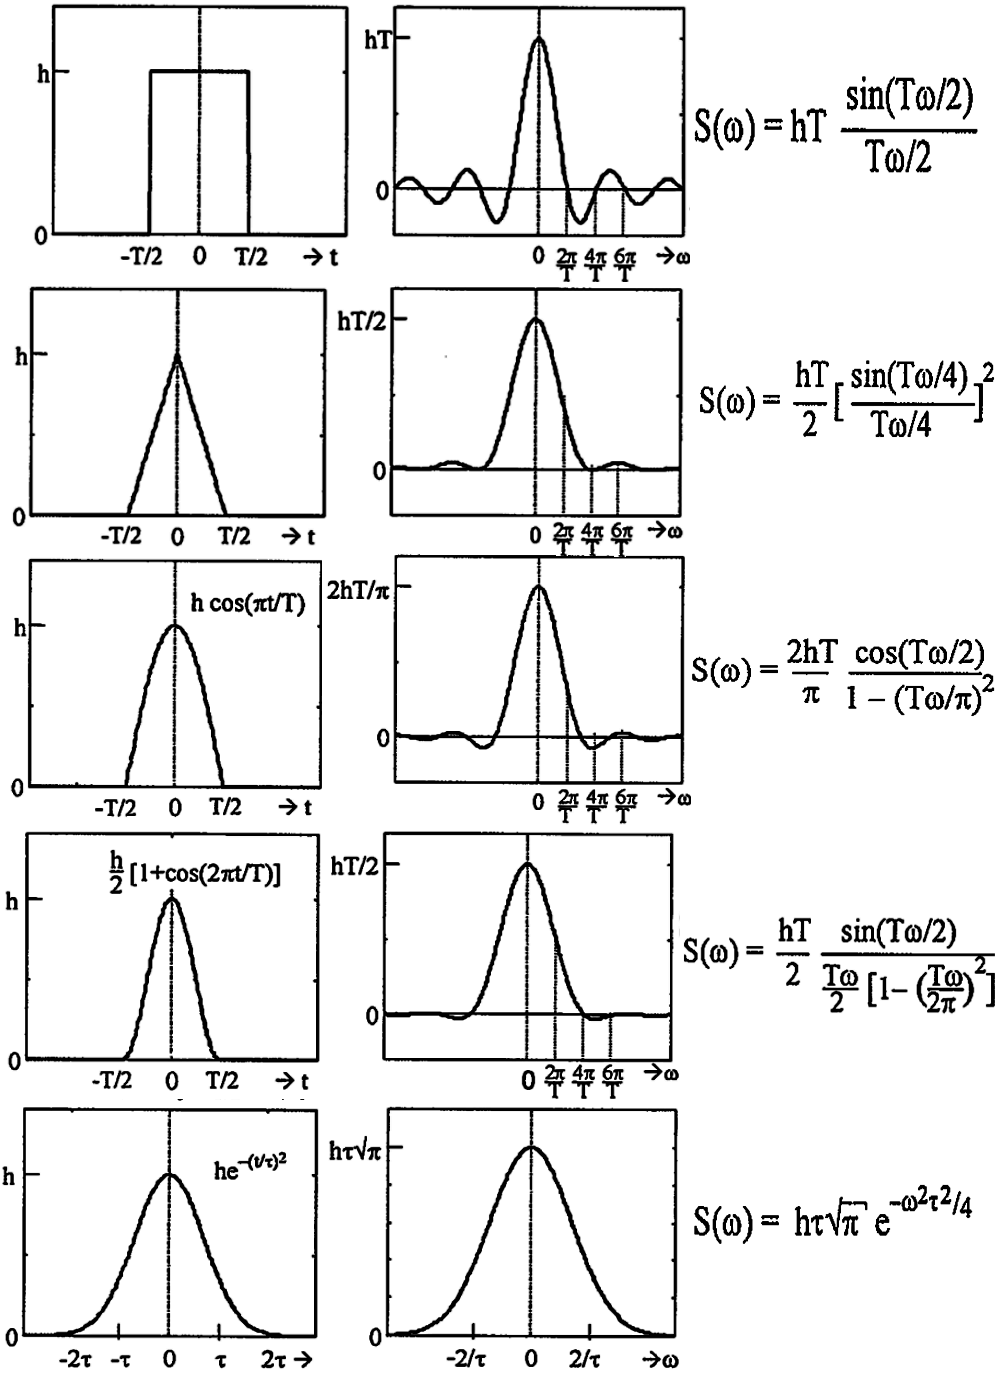
\includegraphics[width=\textwidth,trim= 0cm 0cm 0cm 0cm]{bilder/Transformationen/Fourier-Trafo.png}

\end{minipage}
\begin{minipage}{8.25cm}
	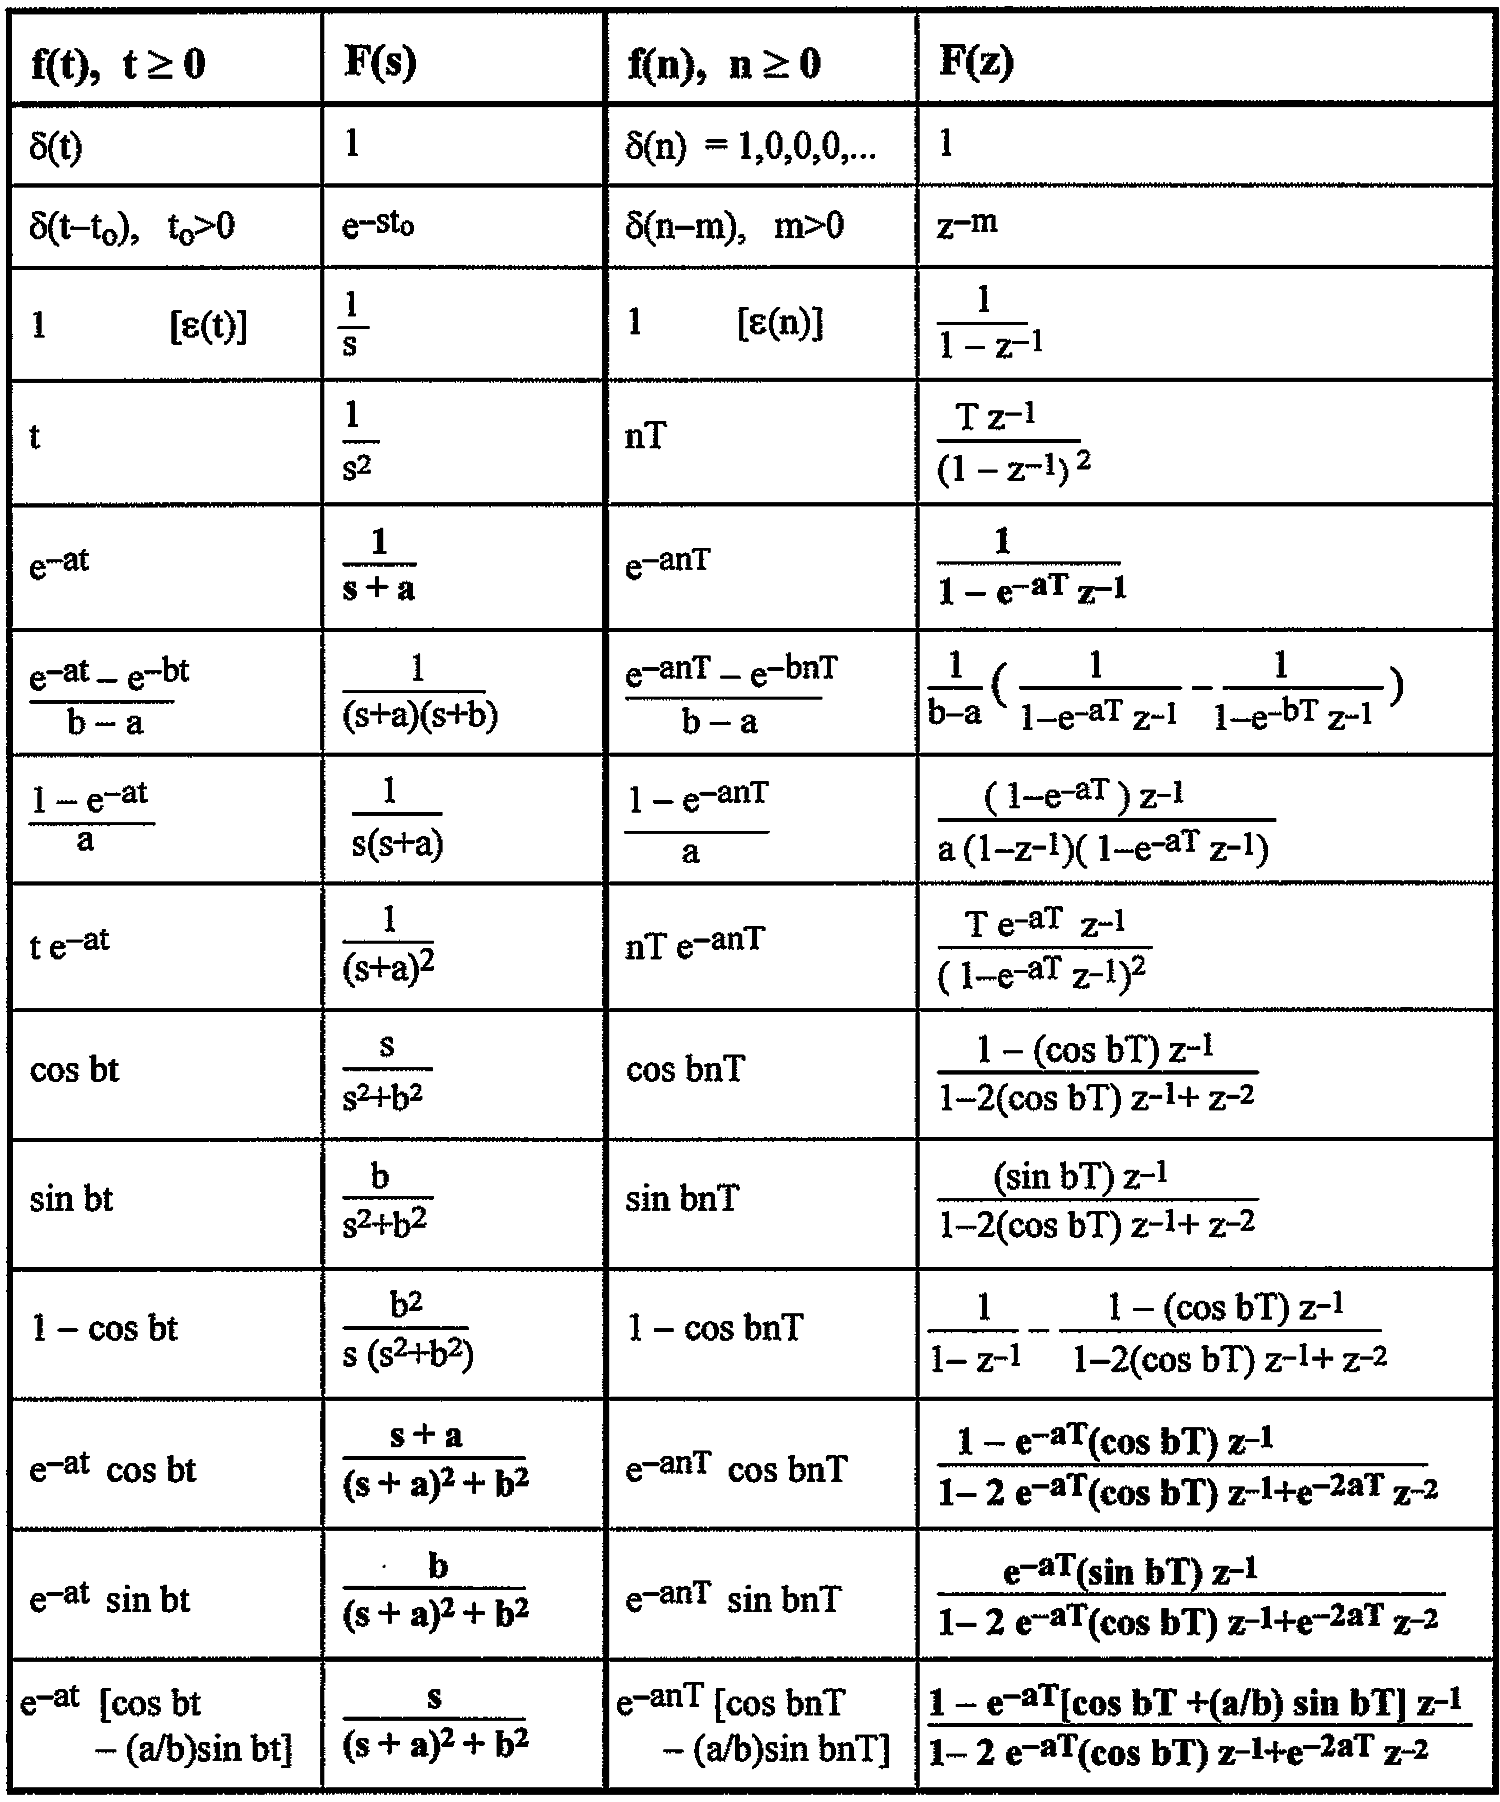
\includegraphics[width=\textwidth,trim= 0cm 0.3cm 0cm 0.45cm]{bilder/Transformationen/Z-Lexikon.png}
	\end{minipage}
	\begin{minipage}{10cm}
	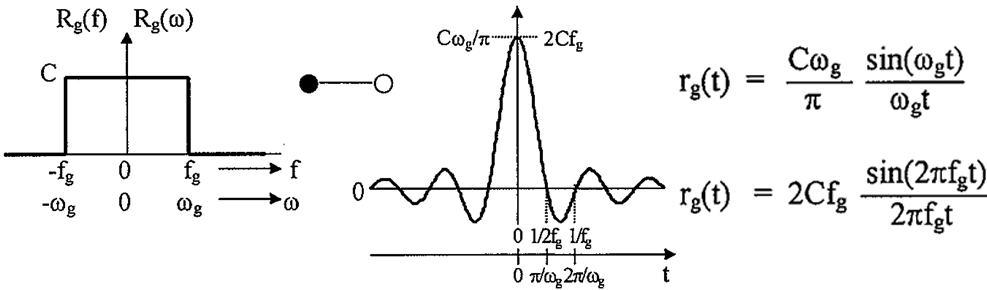
\includegraphics[width=\textwidth,trim= 0cm 0cm 0cm 0cm]{bilder/Transformationen/Rechteck-Sinc.png}
	\textbf{Matrix inversion}\\
	$A^{-1} = \begin{pmatrix}
	a & b \\ c & d \\
	\end{pmatrix}^{-1} =
	\frac{1}{\det(A)} \begin{pmatrix}
	d & -b \\ -c & a \\
	\end{pmatrix}  =
	\frac{1}{ad-bc} \begin{pmatrix}
	d & -b \\ -c & a \\
	\end{pmatrix}\quad$\\
	$A^{-1} = \begin{pmatrix}
	a & b & c\\ d & e & f \\ g & h & i \\
	\end{pmatrix}^{-1} =
	\frac{1}{\det(A)} \begin{pmatrix}
	ei - fh & ch - bi & bf - ce \\
	fg - di & ai - cg & cd - af \\
	dh - eg & bg - ah & ae - bd
	\end{pmatrix}$\\
	\begin{minipage}{4cm}
		\textbf{Trigonometry} \\
		$e^{j\varphi}=\cos(\varphi)+ j \cdot \sin(\varphi) $
		$e^{-j\varphi}=\cos(\varphi)- j \cdot \sin(\varphi) $
		$\cos(x) = \frac{e^{jx} + e^{-jx}}{2}$\\
		$\sin(x) = \frac{e^{jx} - e^{-jx}}{2j}$\\
		$\cos^2(x) = \frac12 + \frac{\cos(2x)}{2}$\\
		$\sin^2(x) = \frac12 - \frac{\cos(2x)}{2}$\\
		$\sin(2x)=2\sin(x)\cdot\cos(x)$\\
		$\sin^2(x)+\cos^2(x)=1$
	\end{minipage}
	\begin{minipage}{5cm}
		\textbf{Determinants} \\
		\footnotesize
		$\det \begin{pmatrix} a & b \\ c & d\\ \end{pmatrix} =
		a d - b c \quad$\\
		$\det \begin{pmatrix} 
		a & b & c \\
		d & e & f \\
		g & h & i  \end{pmatrix}
		= a e i + b f g + c g h \\
		\text{\hspace{2.5cm}} -c e g - f h a - i b d$		\normalsize
	\end{minipage}
\end{minipage}

%\section{Fourier Transformation}
\begin{minipage}{0.85\linewidth}
%\subsubsection{Eigenschaften von Fourier- und Z-Transformation}
\footnotesize 
\renewcommand{\arraystretch}{1.1}
\begin{tabular}{|p{4.3cm}||p{1.8cm}|p{1.8cm}||p{2.2cm}|p{2.4cm}||p{1.9cm}|p{2.6cm}|}
\hline
\textbf{Designation}
  & \multicolumn{2}{|c||}{\textbf{Time domain}}
  & \multicolumn{2}{|c||}{\textbf{Continuous frequency domain}}
  & \multicolumn{2}{|c|}{\textbf{Discrete frequency domain}} \\
  & \textbf{Continuous}
  & \textbf{Discrete}
  & \textbf{Fourier}
  & \textbf{Laplace}
  & \textbf{Discrete FT}
  & \textbf{Z Transform} \\
\hline
\hline
  Linearity 
  & $\alpha\cdot f(t) + \beta\cdot g(t)$
  & $\alpha\cdot f(n) + \beta\cdot g(n)$
  & $\alpha\cdot F(\omega) + \beta\cdot G(\omega)$
  & $\alpha\cdot F(s) + \beta\cdot G(s)$
  & $\alpha\cdot F(n) + \beta\cdot G(n)$
  & $\alpha\cdot F(z) + \beta\cdot G(z)$\\
\hline
  Similarity / Time scaling or reflection about the Y-axis
  &	$f(\alpha t)$ 
  & $f(-n)$
  & $\frac{1}{|\alpha|}F \left (\frac{\omega}{\alpha} \right)$
  & $\frac{1}{\alpha}F \left (\frac{s}{\alpha} \right )$ 
  & $F(-n)$
  & $F(z^{-1})$\\
%\hline
  %Damping
  %& -
  %& $e^{dn} f(n)$
  %& -
  %& - 
  %& -
  %& $F(z e^{d})$ \\
\hline
  Shift in the time domain 
  & $f(t\pm t_0)$ 
  & $f(n \pm n_0)$
  & $e^{\pm j\omega t_0} F(\omega)$
  & $F(s)e^{\pm t_0 s}$ 
  & $e^{\pm j\frac{n}{N}2 \pi n_0} F(n)$
  & $z^{\pm n_0} F(z)$\\
\hline
Shift in the frequency domain 
  & $f(t)e^{\mp\alpha t}$ 
  & $f(n) e^{\mp j \frac{n}{N} 2 \pi n_0}$
  & $F(\omega\pm \alpha)$
  & $F(s\pm\alpha)$ 
  & $F(n \pm n_0)$
  & $F(z \pm n_0)$\\
\hline
Convolution in the time domain 
  &	$f(t) \ast g(t)$
  & $f(n) \ast g(n)$
  & $F(\omega) \cdot G(\omega)$
  & $F(s) \cdot G(s)$
  & $F(n) \cdot G(n)$ 
  & $F(z) \cdot G(z)$ \\
\hline
  Convolution in the frequency domain 
  &	$f(t) \cdot g(t)$
  & $f(n) \cdot g(n)$
  & $\frac{1}{2\pi} F(\omega) \ast G(\omega)$
  & $\frac{1}{2\pi} F(s) \ast G(s)$ 
  & $\frac{1}{N} F(n) \ast G(n)$
  & $\frac{1}{N} F(z) \ast G(z)$\\
\hline
  Derivatives in the time domain / difference formation 
  & $\frac{\partial^n f(t)}{\partial t^n}$ 
  & $\Delta^k f(n)$
  & $(j\omega)^n F(\omega)$
  & $s^nF(s)-s^{n-1}f(0+)-s^{n-2}\frac{\partial f(0+)}{\partial t}-\ldots
 			-s^0\frac{\partial^{n-1} f(0+)}{\partial t^{n-1}}$
  & 
  & $(1-z^{-1})^k F(z)$ \\
\hline
  Derivative in the frequency domain
  & $(-t)^k\cdot f(t)$ 
  & $n f(n)$ 
  & $j^k \frac{-\partial^k F(\omega)}{\partial \omega^k}$
  & $\frac{\partial^k F(s)}{\partial s^k}$
  & 
  & $-z \frac{\partial F(z)}{\partial z}$ \\
\hline 			
  Integration / Summation
  & $\int\limits_{-\infty}^t f(\tau)d\tau$ 
  & $\sum\limits_{n=0}^{k} f(n)$
  & $\frac{F(\omega)}{j\omega}+F(0)\pi\delta(\omega)$
  & $\frac{F(s)}{s}$
  & 
  & $\frac{1}{1-z^{-1}} F(z)$ \\
\hline
  Initial value 
  & $\lim\limits_{t\rightarrow 0} f(t)$ 
  & $f(0)$
  & 
  & $\lim\limits_{s\rightarrow \infty} sF(s)$ 
  & 
  & $\lim\limits_{z \rightarrow \infty} F(z)$ \\
\hline
  Final value
  &	$\lim\limits_{t\rightarrow \infty} f(t)$
  & $\lim\limits_{n\rightarrow \infty} f(n)$
  & 
  & $\lim\limits_{s\rightarrow 0} sF(s)$
  & 
  & $\lim\limits_{z \rightarrow 1} (1-z^{-1}) F(z))$\\
%\hline
  %Stability
  %& -
  %& -
  %& -
  %& Pole in LHP
  %& 
  %& Pole inside unit circle \\
%\hline
  %Causality
  %& -
  %& -
  %& A- \& Causal
  %& Only Causal
  %& 
  %& $\lim\limits_{z \rightarrow \infty} z^{-1} F(z) = 0$ \\
\hline
\hline
  Special
  & \multicolumn{3}{l||}{
      Bessel's theorem \qquad
      $\int\limits_{-\infty}^{\infty}f(t)g^{\ast}(t)dt =
         \frac{1}{2\pi}
         \int\limits_{-\infty}^{\infty}F(\omega)G^{\ast}(\omega)d\omega$}
  & \multicolumn{3}{|l|}{
      Parseval's theorem \qquad
      $W = \int\limits_{-\infty}^{\infty}|f(t)|^2 dt = \frac{1}{2\pi}
      \int\limits_{-\infty}^{\infty}|F(\omega)|^2 d\omega$
    }\\
\hline
\end{tabular}
\end{minipage}
\begin{minipage}{0.2\linewidth}
\textbf{Quadratic Equation:}\\
$a\cdot x^2+b\cdot x +c=0$\\

$x_{1,2}=\frac{-b\pm \sqrt{b^2-4ac}}{2a}$\\

\textbf{Fourier Transform:}\\

$\delta(t)\FT 1$\\
$1\FT 2\pi \delta(\omega)$\\
$\sigma(t)\FT \frac{1}{j\omega}+\pi\delta(\omega)$\\
$\text{sgn}(t)\FT \frac{2}{j\omega}$\\
$e^{\pm j \omega_0 t} \FT 2\pi \delta(\omega \mp \omega_0)$\\
$\sin(\omega_0t)\FT j\pi(\delta(\omega +\omega_0)-\newline\text{\hspace{2.7cm}}\delta(\omega -\omega_0))$\\
$\cos(\omega_0t)\FT \pi(\delta(\omega +\omega_0)+\newline\text{\hspace{2.6cm}}\delta(\omega -\omega_0))$\\
\end{minipage}


%% We don't need this and it does not fit onto the page. The trigonometric relationships are already on this page under ''Trigonometrie'', and the z-transforms are in the z-transform table. 
%% In my opinion the z-transform table should also be updated, because you can barely read it when it's included as a picture and scaled. 
 
% \begin{minipage}{\linewidth}
% \vspace*{-1cm}
% $e^{j\omega}=\cos(\omega) + j \cdot \sin(\omega)$
% \quad
% $\sin(\omega)=\dfrac{e^{j\omega} - e^{-j\omega}}{2j}$
% \quad
% $\cos(\omega)=\dfrac{e^{j\omega} + e^{-j\omega}}{2}$
% \quad
% $1\pm e^{-j\omega T}= (e^{j\frac{\omega}{2} T}\pm e^{-j\frac{\omega}{2} T})\cdot e^{-j\frac{\omega}{2} T}$
% \quad
% $a^n \FT \frac{1}{1-az^-1}$
% \quad
% $a^{|n|} \FT \frac{1-a^2}{(1-az^-1)(1-az)}$
% \quad
% \vspace*{-2cm}
% \end{minipage}


\end{landscape}


\section{Probability Theory}
%\renewcommand{\baselinestretch}{1.25}\normalsize
    \subsection{Combinatorics}
        \begin{minipage}{13.5cm}
        \begin{tabular}{| p{5.5cm} | c | c |}
            \hline
            Type of selection or composition of $k$ from $n$ elements    & \multicolumn{2}{c|}{Number of possibilities}\\
             & without repetitions        & with repetitions\\
             & $(k\leq n)$                & $(k\leq n)$ \\
             \hline
            Permutations & $P_n=n!(n=k)$ &
            $P_n^{(k)}=\frac{n!}{k!}$ \\ & &\\
            Combinations & $C_n^{(k)}=\binom n k$ &
            $C_n^{(k)}=\binom{n+k-1} k$\\
            & &\\
            Variations & $V_n^{(k)}=k!\binom n k$ & $V_n^{(k)}=n^k$\\
            \hline
        \end{tabular}
        \end{minipage}
        \begin{minipage}{5cm}
        $\binom n k$ with TR: \texttt{nCr(n,k)} \hspace{9.3mm}En\\
        \hspace*{19mm} \texttt{Kombinat(n,k)} De
        \end{minipage}
        \begin{list}{$\bullet$}{\setlength{\itemsep}{0cm} \setlength{\parsep}{0cm} \setlength{\topsep}{0.1cm}} 
            \item \textbf{Permutations}: Given are $n$ different objects. Then there are $n!$
            different orders in which these objects can be arranged. \\
            e.g.: $x,y,z;\quad x,z,y;\quad z,y,x;\ldots$
         % \item Permutation is called an arrangement of $n$ elements in a certain
        %       order
            \item \textbf{Combination}: Given are $n$ different objects. Then there are $\binom n k$
            ways to select $k$ objects from them, if the order does not matter. \\
            e.g.: How many different ways are there to select 6 numbers out of 49
            in the lottery?
         % \item Combination is called a selection of $k$ elements from $n$ elements
         %       without considering the order
            \item \textbf{Variation} is called a selection of $k$ elements from $n$
                different elements considering the order
        \end{list}


\vspace{5mm}
    \begin{minipage}{6.8cm}
    \subsection{Probability}
        \begin{tabular}{ll}
            Range of values:
            & ${0}\le{P(A)}\le{1}$\\ \\
            Certain event:
            & $P(\Omega)=1$\\ \\
            Impossible event:
            & $P(\emptyset)=0$
        \end{tabular}
    \end{minipage}
        \begin{minipage}{11.2cm}
        \textbf{Calculation rules}\\
            \begin{tabular}{ll}
                Complementary event:
                &$P(\bar{A})=P({\Omega}\setminus{A})=1-P(A)$\\ \\
                Difference of the events A and B:
                &$P({A}\setminus{B})=P(A)-P({A}\cap{B})$\\ \\
                Union of two events:
                &$P({A}\cup{B})=P(A)+P(B)-P({A}\cap{B})$
            \end{tabular}
        \end{minipage}
\vspace{1mm}


	\subsection{Laplace Events}
		In a finite probability space $\Omega$, all
		elementary events have the same probability.
		\begin{center}
		$P(A)=\dfrac{\left| A\right|}{\left|\Omega\right|}$
		\end{center}

	\subsection{Independent Events}
		Independent events $A$ and $B$ are present when:\\
		\hspace*{8mm} $P(A\mid B)=P(A)$ \hspace{4mm} and \hspace{4mm}
		$P(B\mid A)=P(B)$\\
		is satisfied. For them, it applies\\
		\hspace*{8mm} $P(A\cap B)=P(A)P(B)$\\
		The fact that A has occurred has no influence on the 
		probability of B.\vspace{1mm}


	\subsection{Conditional Probability}
		The probability of the occurrence of event $A$ given that
		event $B$ has already occurred.
		\begin{center}
		$P(A\mid B)= \dfrac{P(A\cap B)}{P(B)}=\underbrace{\frac{P(A)\cdot
		P(B)}{P(B)}=P(A)}_{\text{only if independent}}$ 
		\end{center}


	\subsection{Bayes' Theorem}
		\begin{tabular}{ll}
		$P(B\mid A)=P(A\mid B) \cdot\dfrac{P(B)}{P(A)}$\vspace{1mm}
		\end{tabular}


	\subsection{Total Probability}
		\begin{tabular}{ll}
		$P(A)=\sum\limits_{i=1}^N P(A\mid G_i)\cdot P(G_i)$
		\end{tabular}


	\subsection{Probability Distribution}

		\subsubsection{Distribution Function}
			\renewcommand{\arraystretch}{1.5}
			\begin{tabular}[]{|l|l|}
				\hline
				\textbf{discrete} & \textbf{continuous}\\
				\hline
				\hline
				$P(X\leq x)=F(x)=\sum\limits_{k=-\infty}^x p_k$ &
				$P(X\leq x)=F(x)=\int\limits_{-\infty}^x\varphi(\tilde{x})d\tilde{x}$\\
				$P(X>x)=1-P(X\leq x)$ & 
				$P(X>x)=1-P(X\leq x)$\\     
				   
				$P(\alpha_1 \le X \leq \alpha_2)=F(\alpha_2)-F(\alpha_1)=\sum\limits_{k=\alpha_1}^{\alpha_2} p_k$ &          
				$P(\alpha_1 \le X \leq \alpha_2)=F(\alpha_2)-F(\alpha_1)=\int \limits_{\alpha_1}^{\alpha_2}\varphi(\tilde{x})d\tilde{x}$\\
			
				$F_{x_1,x_2}(\alpha_1,\alpha_2)=P(\alpha_1 \le X_1 , \alpha_2\leq X_2)$&
				$F_{x_1,x_2}(\alpha_1,\alpha_2)=P(\alpha_1 \le X_1 , \alpha_2\leq X_2)$\\
				\hline
			\end{tabular}
			\renewcommand{\arraystretch}{1}
	
			\textbf{Properties}
					$$\boxed{\mathbb{D}(F) = \mathbb{R}} \qquad \boxed{\mathbb{W}(F)
					\in[0,1]} \qquad \boxed{F(-\infty)=0} \qquad  \boxed{F(\infty)=1}
					\qquad \boxed{F(x) \text{ is monotonically increasing}}$$
	
	
		\subsubsection{Probability Density }
			\begin{tabular}{p{7.3cm}p{8.5cm}}
			$\varphi(x)=F'(x)$ &Density function or probability density\\
			$\varphi_{x_1,x_2}(\alpha_1,\alpha_2)=\frac{\delta^2}{\delta_{x_1}\delta{x_2}}F_{x_1,x_2}(\alpha_1,\alpha_2)$ &Density function or probability density with multiple variables\\
			
			\multirow{2}{11cm}{At jump points of F(x): }\\
			\multirow{2}{11cm}{$\varphi(x) = $ Dirac with the weight of the jump height}
			\end{tabular}
	
	
		\subsubsection{Calculation Rules for $\varphi$ and $F$ }
			\begin{minipage}{11cm}
				\begin{tabular}{ll}
				Given: &X, Y random variables\\
				&$\varphi_x$, $\varphi_y$ known\\
				\end{tabular}
	 
				\begin{tabular}{p{6cm}p{6cm}}
				Distribution Function: &Density:\\
				$F_{x+a}(x)=F_x(x-a)$  &$\varphi_{x+a}(x)=\varphi_x(x-a)$\\
				$F_{\lambda x}(x)=F_x(\frac{x}{\lambda})$ &$\varphi_{\lambda
				x}(x)=\varphi_x(\frac{x}{\lambda})\frac{1}{\lambda}$\\
				$F_{x+y}(x)=F_x\ast\varphi_y(y)=F_y\ast\varphi_x(x)$ &
				$\varphi_{x+y}(x)=\varphi_x\ast\varphi_y(x)$\\
				$F_{\sqrt{x}}(x)=F_x(x^2)$ &
				$\varphi_{\sqrt{x}}(x)=2x\varphi_x(x^2)$\\
				$F_{x^2}(x)=F_x(\sqrt{x})$ &
				$\varphi_{x^2}(x)=\frac{1}{2}x^{-\frac{1}{2}}\varphi_x(\sqrt{x})$
				\end{tabular}
			\end{minipage}
			\begin{minipage}{7cm}
				\textbf{Algorithm Example}
				\begin{tabular}{ll}
				1. Apply definition of $F$: $F_{\lambda x}(x)=P(\underbrace
				{\lambda X\leq x}_{*})$\\ 
				2. Reformulate condition *: $P(X \leq
				\frac{x}{\lambda})=F_x(\frac{x}{\lambda})$\\ 
				3. for density: $\frac{d}{dx}$\\
				\vspace{3mm}
				$\varphi_{\lambda x}(x)=\frac{d}{dx}F_{\lambda
				x}(x)=\frac{d}{dx}F_x(\frac{x}{\lambda})=
				\varphi_x(\frac{x}{\lambda})\frac{1}{\lambda}$
				\end{tabular}
				\vspace{10mm}
			\end{minipage}


		\subsubsection{Expected Value}
			Let $X$ be a function on $\Omega$, and suppose $\Omega$ can be divided into finitely many
			events, on which $X(\omega)$ is constant, $A_i$, then the expected value of $X$\\
			$Expected value = \sum Value \cdot Probability$\\
			$E(X)=\sum\limits_{i=0}^n \underbrace{a_i}_{\text{Value}}\cdot \underbrace{P(X=a_i)}_{\text{Prob.}}=\int\limits_{-\infty}^\infty \alpha \cdot \varphi_x(x)d\alpha$\\
			$E(y)=E(g(x))=\int\limits_{-\infty}^\infty g(\alpha) \cdot \varphi_x(x)d\alpha$ \hspace{2mm} for $y=g(x)$\\
			
	
			\textbf{Calculation Rules}\\
				\begin{tabular}{ll}
				$E(X+Y)=E(X)+E(Y)$\\
				$E(\lambda X + \mu)=\lambda \cdot E(X) + \mu$ & $\lambda, \mu \in \mathbb{R}$\\
				$E(XY) = E(X)\cdot E(Y)$ & if X,Y are independent\\
				\end{tabular}
	
      
		\subsubsection{Variance}

			\begin{tabular}{ll}
			$var(x)=\sigma ^2=E[(X-E(X))^2]=E(X^2)-E(X)^2$\\$=\int\limits_\infty^\infty(\alpha - E(x))^2\varphi_x(\alpha)d\alpha$\\
			\end{tabular}
			
			\textbf{Calculation Rules}\\
				\begin{tabular}{ll}
				$var(\lambda X)=\lambda^2 var(X) \qquad $ $\lambda, \mu \in
				\mathbb{R}$\\ 
				$var(X_1+X_2+\ldots+X_n) \neq var(n X)$ \\
				$var(X+Y)= \begin{cases}
								var(X)+var(Y)
								&   \text{(X,Y independent)}\\                     
								var(X) + var(Y) + 2 \cdot cov(X,Y) 
								&   \text{(X,Y dependent)}\\
							\end{cases} $ \\
				$var(X Y)= var(Y)var(X)+var(Y)E(X)^2+var(X)E(Y)^2$
				\end{tabular}
	
		\subsubsection{Correlation}
		\begin{tabular}{ll}
        $r_{xy}=E(XY^*)$
        \end{tabular}
		\subsubsection{Covariance}
		\begin{tabular}{ll}
			$c_{xy}=cov(X,Y)=E((x-E(X))(y-E(Y)))$\\$=E(XY^*)-E(X)E(Y)=\underbrace{0}_{\text{if X,Y are independent}}=
			\underbrace{r_{xy}}_{\text{if X,Y are mean-free}}$
		\end{tabular}
        \subsubsection{Correlation Coefficient}
		$\rho_{xy}=\frac{E((X-m_x)\cdot(Y-m_y)^*)}{\rho_x \rho_y}$\\
		$|\rho_{xy}\leq 1|$ \\ 
		\textbf{Independent}\\
        Two random variables are statistically independent if the probability density function is separable: \\
        $\varphi_{xy}(\alpha, \beta) = \varphi_x(\alpha)\varphi_y(\beta) \Longrightarrow$ also $E(XY)=E(X)E(Y)$ \\
        If the variables are additionally uncorrelated, it holds that: $Var(X+Y) = Var(X) + Var(Y)$


		\subsubsection{Moment Generating Function}
        The moment generating function is a representation of all moments of a distribution. 
        $\Phi(t)=E(e^{tX})=\int\limits_{-\infty}^\infty e^{tx} \cdot \varphi(x) dx$ or $= \sum\limits_{i=1}^{\infty}e^{tx_i} \cdot P(X=x_i)$  \\
        $\Phi(t)$ is called the moment generating function because: \\
        $\frac{d^n}{dt^n}\Phi(t)=\int\limits_{-\infty}^\infty x^n \cdot e^{tx} \cdot \varphi(x) dx$ or $= \sum\limits_{i=1}^{\infty} x_i^n \cdot e^{tx_i} \cdot P(X=x_i)$\\
        for $\frac{d^n}{dt^n}\Phi(0)=\int\limits_{-\infty}^\infty x^n \cdot \varphi(x) dx$ or $= \sum\limits_{i=1}^{\infty} x_i^n \cdot P(X=x_i) = E(X^n)=\mu_n $\\

        If $\Phi_x(t) = \Phi_y(t)$ then $F_x(x)=F_y(x)$. This means a probability distribution can be uniquely associated with a moment generating function.


    \subsubsection{Various Probability Density Functions}
        \textbf{Gaussian Distribution/ Normal Distribution}\\
        \begin{minipage}{10cm}
        Many small, independent random variables accumulate to form a
        normally distributed random variable.\\
         $\varphi(x)=\frac{1}{\sqrt{2
        \pi}\sigma}\cdot e^{-\frac{(x-\mu)^2}{2\sigma^2}} = N(\mu ; \sigma^2) $\\ 
        $F(x)=\frac{1}{\sqrt{2
        \pi}\sigma}\cdot \int\limits^{x}_{-\infty}{e^{-\frac{(\tilde{x} -\mu)^2}{2\sigma^2}}} $ \\
        \textbf{Standardization}\\
        Expected Value: $E(X)=\mu$ \hspace{4mm}(=0 in Standard normal dist.)\\ 
        Variance \hspace{11.5mm}: $var(X)=\sigma^2$ (=1 in Standard normal dist.)\\ \\
        $x=\dfrac{X-\mu}{\sigma}$ \hspace{5mm} $x$ from table
        \end{minipage}
        \hspace{5mm}
        \begin{minipage}{7.5cm}
        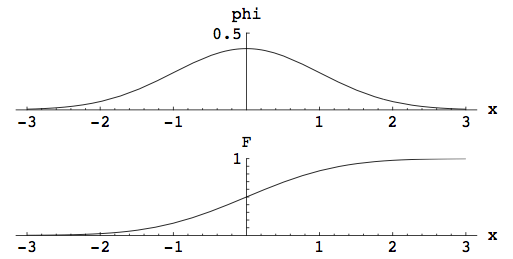
\includegraphics[width=7.5cm]{bilder/normalverteilung.png}
        Density function (above) and distribution function (below) of the normal distribution. 
        \end{minipage} \\ \\
        $ 68\% $ of the values lie within the interval $[ \mu - \sigma, \mu + \sigma]$, 
        $95\% $ in $[ \mu - 2\sigma, \mu + 2\sigma]$,    
        $99.7\% $ in $[ \mu - 3\sigma, \mu + 3\sigma]$\\\\
        \textbf{ Normal Distribution with Multiple Variables}\\
        $\varphi_{x,y}(\alpha,\beta)=\frac{1}{2\pi \sigma_x \sigma_y \sqrt{1-\rho_{xy}^2}}
            e^{-\frac{1}{2(1-\rho_{xy})^2} + \frac{(\alpha - m_x)^2}{\sigma_x^2} 
            - 2\rho_{xy}\frac{(\alpha - m_x)\beta - m_y)^2}{\sigma_x \sigma_y} + \frac{(\beta - m_y)^2}{\sigma_y^2}}$\\
            $\varphi_x(\textbf{x})=\frac{1}{(2\pi)^{\frac{n}{2}}|\textbf{C}_x|^{\frac{1}{2}}}\cdot 
            e^{-\frac{1}{2}(\textbf{x} - \textbf{m}_x)^T \textbf{C}_x^{-1} (\textbf{x} - \textbf{m}_x)}$ with \\
            $\textbf{m}_x=[E(x_1), E(x_2), \ldots, E(x_n)]^T$ and covariance matrix $\textbf{C}_x$; $c_{ij} = E((x_i-E(x_i)(x_j-E(x_j))))$ \\
        \textbf{Calculation Rule for the Normal Distribution with Multiple Variables}
        \begin{itemize}
          \item if $z=a x + b y$ then \\
          $m_z =  a m_x + b m_y$\\
          $\sigma_z^2 = a^2\sigma_x^2 + b^2\sigma_y^2+2ab\sigma_x\sigma_y$
          \item if x and y are uncorrelated, then \\
                $f_{x,y}(\alpha, \beta) = \varphi_x(\alpha)\varphi_y(\beta)$ meaning x and y are also statistically independent.
          \item The optimal nonlinear estimator for the values $\mu$ and $\sigma$ is the same as the linear estimator.
        \end{itemize}


		\subsection{Random Processes}
		\begin{minipage}{10.3cm}
			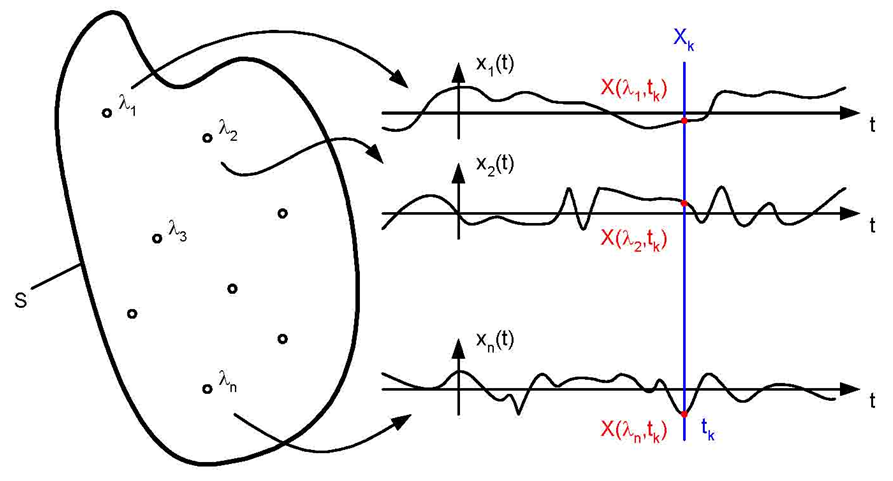
\includegraphics[width=10cm]{bilder/zufallsprozess.png}
		\end{minipage}
		\begin{minipage}{8.5cm}
			In a \textbf{random process}, each \textbf{outcome} \boldmath$\lambda$ from 
			the \textbf{outcome space} $S$ is assigned a \textbf{deterministic} \textbf{function} $x(\lambda, t)$
			\unboldmath. \\
			Random processes describe a deterministic time function triggered by the outcome of
			a random experiment. e.g., $sin(\omega t + X)$ where X is a random variable assigned from the event space at the beginning.\\
			Temporally \textbf{randomly occurring functions} can also be seen as \textbf{deterministic functions} 
			\textbf{interpreted} in such a way that the observer never knows which specific function $x_\lambda(t)$
			is present.  \\ \\
			For comparison: In the case of random variables, each elementary event is assigned a number. 
		\end{minipage} 
		\vspace{0.5cm} \\

		\subsubsection{Statistical Averages (Ensemble Averages)}
		The statistical averages are a function of time $t$, as they are averages over the
		ensemble (entire outcome space). Here, all deterministic functions are averaged at a
		specific time $t$.

		\renewcommand{\arraystretch}{1.4}
		\begin{tabular}[c]{ p{4.5cm}  p{13.5 cm}  }
			\textbf{Expected Value}:   &  $\mu_{x}(t) = E\left[X(t)\right] =
				  \int\limits_{-\infty}^{+\infty} x \cdot f_{x}(x;t)\;dx$ or $=\frac{1}{N}\sum\limits_{i=1}^{N}x_i(n)$ \\
			\textbf{Expected Value of a Deterministic Signal}:& $\mu_f(t) = E(f(t))=f(t)$\\
			\textbf{Variance}: &         $\sigma_x^2(t)=E((x(t)-\mu_x(t))^2)=c_x(t_1,t_1)$
		\end{tabular}
		\renewcommand{\arraystretch}{1}


		\subsubsection{Stationarity}
		A stationary process does not change its statistical properties over time. \\
		
		\textbf{Strict Sense Stationarity (SSS)}\\
		In a strictly stationary process, the n-dimensional probability densities remain constant over
		time. That is, the \textbf{statistical properties} and thus the probability densities are the
		\textbf{same at all times}.
		$$ f_x(x_1, x_2, \ldots, x_n; t_1, t_2, \ldots, t_n) =
				f_x(x_1, x_2, \ldots, x_n; t_1+c, t_2+c, \ldots, t_n+c) \qquad \forall (c,n \in
				\mathbb{R})$$
		
		\textbf{Wide Sense Stationarity (WSS) - Second-order Stationarity}\\
		In a weakly stationary process, the statistical properties are \textbf{not the same at every
		moment in time}, however, they are \textbf{not dependent on an absolute} point in time, but
		rather on the \textbf{difference} ($\tau$) \textbf{between two points in time} ($t_1, t_2$).  \\ 
		$$ f_x(x_1, x_2; t_1, t_2) = f_x(x_1, x_2; t_1+c, t_2+c) \qquad \forall (c \in
				\mathbb{R})$$
		\renewcommand{\arraystretch}{1.4}
		\begin{tabular}[c]{ p{3.3cm}  p{6.5cm} p{8cm} }
			\textbf{Mean}:     &  $E[X(t)] = \mu_{x} = \text{const.}$  
									& remains constant over time\\ 
			\textbf{Quadratic Mean}:    &  $E[X^{2}(t)] = r_{x}(0)$  \\ 
			\textbf{Autocorrelation}:   &   $r_{xx}(t_{1},t_{2}) = r_{x}(\tau)$
			& \multirow{2}{8cm}{only \textbf{dependent} on the \textbf{time difference} $(\tau = t_2 - t_1)$ and \textbf{not directly} on
			 the \textbf{time} $t$} \\
			 \textbf{Autocovariance}:        & $ c_{xx}(t_{1},t_{2}) = r_{x}(\tau) - \mu_{x}^{2} = c_{xx}(\tau)$ \\
		\end{tabular}
		\renewcommand{\arraystretch}{1}
		 
		A random process is always a WSS process as long as the expectation is constant and the autocorrelation function is only a function of $\tau$, i.e., both 
		statistical parameters are independent with respect to a temporal shift.    
		Every strictly stationary process is also weakly stationary, but not vice versa. 
		
		\subsubsection{Time Averages (Time Means)}
		Here, the respective deterministic functions (sample functions) are averaged over time.
		If the time average is calculated over the entire random process, then the
		time averages are \textbf{random variables}, i.e., the following two expressions are
		dependent on which function is used (hence the index $_i$).
		
		\begin{tabular}[c]{ p{4cm}  p{14.5cm}  }
			\textbf{Mean}:    &  
			$\overline{x_{i}} = \left\langle x_{i}(t) \right\rangle = 
				   \lim\limits_{T \rightarrow \infty}
					 \frac{1}{T} \int\limits_{-\frac{T}{2}}^{+\frac{T}{2}} x_{i}(t) \; dt$ \\
			   \textbf{Autocorrelation}:  &   
			$\overline{r}_{x_{i}x_{i}}(\tau) = \left\langle x_{i}(t) \cdot x_{i}(t+\tau) \right\rangle = 
				   \lim\limits_{T \rightarrow \infty}
					 \frac{1}{T} \int\limits_{-\frac{T}{2}}^{+\frac{T}{2}} x_{i}(t) \cdot x_{i}(t + \tau) \; dt$\\
			\multicolumn{2}{l}{If the \textbf{process is stationary}, the following applies: } \\
			\textbf{Mean}:    &  
			$E[\overline{x}] = 
				   \lim\limits_{T \rightarrow \infty}
					 \frac{1}{T} \int\limits_{-\frac{T}{2}}^{+\frac{T}{2}} E[x(t)] \; dt = 
					 \frac{1}{T} \int\limits_{-\frac{T}{2}}^{+\frac{T}{2}} \mu_{x} \; dt = \mu_{x}$  \\
			   \textbf{Autocorrelation}:  &   
			$E[\overline{r}_{xx}(\tau)] = 
				   \lim\limits_{T \rightarrow \infty}
					 \frac{1}{T} \int\limits_{-\frac{T}{2}}^{+\frac{T}{2}} E[x(t)x(t+\tau)] \; dt =
					 \frac{1}{T} \int\limits_{-\frac{T}{2}}^{+\frac{T}{2}} r_{xx}(\tau) \; dt = r_{xx}(\tau)$\\
		\end{tabular}
		\renewcommand{\arraystretch}{1}
		

		\subsubsection{Ergodicity}
		A stationary process is also ergodic if the \textbf{time averages} correspond to the
		\textbf{statistical averages}.
		
			\begin{minipage}{5cm}
				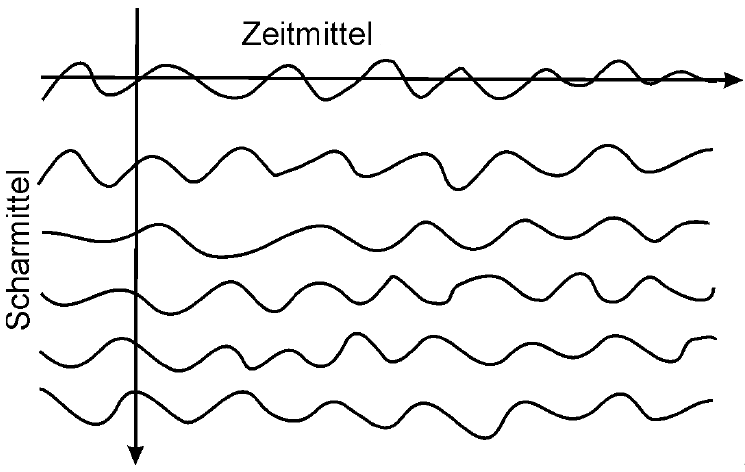
\includegraphics[width=4.5cm]{bilder/zeit-scharmittel.png}
			\end{minipage}
			\begin{minipage}{13.5cm}
		
			\begin{tabular}{ll}
				\multicolumn{2}{l}{Only in ergodic processes it necessarily holds:} \\ \\
			  $E[X(t)] = \overline{x} = \left\langle x(t) \right\rangle$ & DC-Level \\
			  $E[X(t)]^{2} = (\overline{x})^{2} = \left\langle x(t) \right\rangle^{2}$ & DC-Power \\
			  $E[X^{2}(t)] = r_{xx}(0) = \overline{x^{2}} = 
							 \left\langle x^{2}(t) \right\rangle $ & Total Power \\
			  $\sigma_{x}^{2}(t) = \left\langle x^{2}(t) \right\rangle 
								   - \left\langle x(t) \right\rangle^{2}$ & AC-Power \\
			  $\sigma_{x}(t) = \overline{\sigma}_{x}$ & RMS-Level (Effective value) of the AC signal\\
			\end{tabular} \\
			\end{minipage}
		
		
		\subsubsection{Comparison Stationary - Ergodic}
		\textbf{Swarm of mosquitoes:}\\
		\textbf{Ergodic:} If all mosquitoes fly together in a swarm, then averaged over time (Time average), each mosquito flies as fast as the entire swarm on average (Ensemble average), otherwise, the swarm could not stay together. \\
		\textbf{Stationary:} If a mosquito is sick and cannot keep up with the swarm, it flies alone and, above all, slower. Thus, its average speed (Time average) is not equal to that of the swarm (Ensemble average), so it arrives later at the destination. \\
		\textbf{Neither:} If the mosquitoes fly slower after the start, the average speed of the swarm (Ensemble average) is not constant.
		
		\textbf{School grades:}\\
		\textbf{Ergodic:} All students would have to have the same report card grade (Time average) and moreover, this grade would also have to correspond to the class average (Ensemble average) of the individual exams. \\
		\textbf{Stationary:} The class average (Ensemble average) is the same for every exam, but there are students of varying strengths with different report card grades (Time average). \\
		\textbf{Neither:} The class average (Ensemble average) is always different.
		
		\textbf{Thermal noise:} \\
		This is \textbf{ergodic} at a constant temperature.


		\subsubsection{Correlations and Power Spectra}
		Formulas in this section apply to \textbf{stationary} processes. \\
		
		\renewcommand{\arraystretch}{1.6}
		\begin{tabular}[c]{ p{3.5cm}  p{6cm} p{7.5cm} }
			\textbf{Autocorrelation}:     &  
			\multicolumn{2}{l}{$r_x(t_1,t_2)=r_x(t_1-t_2)=r_x(\tau)=r_{xx}(\tau) = E[X(t)X(t+\tau)]$} \\
			  &    $\mid \! r_{xx}(\tau) \! \mid \leq r_{xx}(0) = E[X^{2}(t)]$ 
			& $r_{xx}(-\tau) = r_{xx}(\tau) \quad$ (even, Fourier transform becomes real)\\
		  \textbf{Cross-correlation}:&     
			$r_{xy}(\tau)=r_{xy}(\tau) = E[X(t)Y(t+\tau)]$  
			& $r_{xy}(-\tau) = r_{yx}(\tau) \quad$ (Order of indices!) \\
			& $|r_{xy}(\tau)| \leq \frac{1}{2} \left[ r_{xx}(0)+r_{yy}(0)\right] $
			& $|r_{xy}(\tau)|  \leq \sqrt{r_{xx}(0)r_{yy}(0)}$ \\
		   \textbf{Autocovariance }:     &  \multicolumn{2}{l}{$c_{xx}(t_{1},t_{2}) =
				  E\left[ \left( X(t_{1})-\mu_{x}(t_{1})\right) \cdot
						  \left( X(t_{2})-\mu_{x}(t_{2})\right) \right] =
				  r_{xx}(t_{1},t_{2}) - \mu_{x}(t_{1}) \cdot \mu_{x}(t_{2})=$}\\    
			&\multicolumn{2}{l}{$c_x(\tau)=c_{xx}(\tau) = E\!\left[ \left( X(t)      - E[X(t)]      \right) \cdot
										  \left( X(t+\tau) - E[X(t+\tau)] \right) \right] =
								r_{xx}(\tau) - \mu^{2}_{x} $} \\
			\textbf{Cross-covariance}:     & \multicolumn{2}{l} {$c_{xy}(t_{1},t_{2}) = 
				  E\left[ \left( X(t_{1})-\mu_{x}(t_{1})\right) \cdot
						  \left( Y(t_{2})-\mu_{y}(t_{2})\right)^* \right] =
				  r_{xy}(t_{1},t_{2}) - \mu_{x}(t_{1}) \cdot \mu_{y}(t_{2})=$}\\    
			&\multicolumn{2}{l}{$c_{xy}(\tau) = E\!\left[ \left( X(t)      - E[X(t)]      \right) \cdot
										  \left( Y(t+\tau) - E[Y(t+\tau)] \right) \right] =
								r_{xy}(\tau) - \mu_{x}\mu_{y} $}\\
			& \multicolumn{2}{l}{Random processes are considered \textbf{uncorrelated} if $c_{xy}(\tau) = 0$}
		\end{tabular}
		\renewcommand{\arraystretch}{1}
		
		\textbf{Spectral Power}\\
		The autocorrelation function $r_{xx}(\tau)$ and power spectral density $P_{xx}(\omega)$ form a
		Fourier-\textbf{transform pair}. \\ The power spectral density can be interpreted as the \textbf{average power per frequency band} and is
		defined as follows:                             
				$$ P_{xx}(\omega) = E\left[ \lim\limits_{T \rightarrow \infty}
											\frac{1}{T} \cdot \mid\! X(\omega) \!\mid^{2}\right]                          
									= \int\limits_{-\infty}^{+\infty} r_{xx}(\tau) \cdot e^{-j\omega\tau} \; d\tau 
									\qquad \IFT \qquad
				r_{xx}(\tau)   = \frac{1}{2\pi} \int\limits_{-\infty}^{+\infty} 
									 P_{xx}(\omega) \cdot e^{j\omega\tau} \; d\omega$$ 
				or:
				 
				$$P_{xx}(z) = \sum\limits_{k=-\infty}^{\infty} r_{xx}(k)z^{-k}\qquad \IFT \qquad 
				r_{xx}(k)=\frac 1{2\pi} \int \limits_{-\pi}^{\pi} P_{xx}(e^{jw})e^{jkw}dw \qquad 
				r_{xx}(0) =\frac 1{2\pi} \int \limits_{-\pi}^{\pi} P_{xx}(e^{jw})dw = \lim\limits_{z \rightarrow 0} P_{xx}(z)$$
									 
		$P_{xx}(\omega)$ is purely real, symmetric $(P_{xx}(z)=P_{xx}^*(\frac{1}{z^*}))$ and $\geq 0$. \\
		Cross-correlations ($r_{yx}(\tau), r_{xy}(\tau)$) and cross-spectral densities ($P_{yx}(\tau),
		P_{xy}(\tau)$) form a Fourier-transform pair.
		\begin{center}
		$ r_{yx}(\tau) \FT P_{yx}(\omega) \qquad \qquad r_{xy}(\tau) \FT P_{xy}(\omega)  $
		\end{center}
		Since autocorrelations are definitely non-causal (defined also for negative time values), the bilateral z-transform must be applied.
		
		The eigenvalues of the autocorrelation matrix have the following limitation:\\
		$$\min\limits_\omega P_{xx}(z)\leq \lambda_i \leq \max\limits_{\omega}P_{xx}(z)$$
		

		\subsubsection{Autocorrelation Examples}
		\begin{tabular}{|l|l|l|}
			\hline
				White Noise
				& $r_{xx} (n) = \frac {N_0}{2} \delta(n) \FT P_{xx}(z)= \frac {N_0}{2};\hspace{0.25cm}$ & all z\\
			\hline
				First-Order Process
				& $r_{xx} (n) = P_s \cdot a^{|n|} \FT P_{xx} (z) = P_s \cdot \frac {1-a^2}{(1-az^{-1})(1-az)}$ & for $a<|z| < \frac{1}{a}$\\
			\hline
				
				& $r_{xx} (n) = a^n(u(n) - u(n-N)) \FT P_{xx} (z) = \frac{1-a^Nz^{-N}}{1-az^{-1}}$ & for $|z| > 0$\\
			\hline
				
				& $r_{xx} (n) = a^n \cdot u(n) \FT P_{xx} (z) = \frac{1}{1-az^{-1}}$ & for $|z| > a$\\
			\hline
				
				& $r_{xx} (n) = -a^n \cdot u(-n-1) \FT P_{xx} (z) = \frac{1}{1-az^{-1}}$ & for $|z| < a$\\
			\hline
				Binary Data Signal
				& $r_{xx} (0) = P_s = A_1^2p_1 + A_0^2 p_0 $ &\\
				&$r_{ss} (|n| < T) = $ linear transition from $r_{ss}(0)$ to $r_{ss} (|n| = T)$ &\\
				& $r_{xx} (|n| \geq T) = P_s = A_1^2p_1^2 + A_0A_1p_0p_1 + A_1A_0p_1p_0 + A_0^2p_0^2$ &  \\
			\hline
				Superimposed Signals
				& $r_{gg\pm}(n) = r_{ss}(n) + r_{sf}(n) + r_{sf}(-n) + r_{ff}(n) $ &\\
				$g_\pm(t) = s(t) \pm f(t)$
				&  $\FT P_{g+}(\omega) = P_{s}(\omega) + P_{f}(\omega) \pm 2 \text{Re} \{P_{sf}(\omega) \}$ &\\ 
			\hline
		\end{tabular} 
		\vspace{-0.5cm}
		\subsubsection{Numerical Calculation}
		\begin{tabular}{|l|l|}
			\hline
				\multicolumn{2}{|l|}{\textbf{Numerical Calculation}} \\
			\hline
			Autocorrelation
				& $\hat{r}_{xx} (n) = \frac 1 N \sum\limits_{m=0}^{N-1} s(m ) s[(m+n) ] 
											 = \frac 1 N \sum\limits_{m=0}^{N-1} s[(m-n) ] s(m ) \DFT \hat{P}_{xx}(z)$ \\
			\hline
			Cross-correlation
				& $\hat{r}_{xy} (n ) = \frac 1 N \sum\limits_{m=0}^{N-1} s(m ) f[(m+n) ] 
											 = \frac 1 N \sum\limits_{m=0}^{N-1} s[(m-n) ] f(m ) \DFT \hat{P}_{xy}(z) $ \\
			\hline
			Power Spectral Density 
				& $\hat{P}_{xx}(z) = \frac 1N \left|S_T(z)\right|^2 \IDFT \hat{r}_{xx} (n )
					\qquad \text{with} \quad S_T(z) \IDFT s(n)$\\
			\hline
			Cross Power Spectral Density 
				& $\hat{P}_{xy}(z) = \frac 1N S_T^*(z) F_T(z) \IDFT \hat{r}_{xy} (n )
				\qquad \text{with} \quad F_T(z) \IDFT f(n)$\\

			\hline
		\end{tabular}


		\subsubsection{Transmission of Random Processes through LTI Systems}
		A random process is transmitted through an LTI system. \hspace{2cm} $Y(t) = L[X(t)] \Rightarrow
		Y(t) = h(t) \ast X(t)$ \vspace{0.3cm}\\
		\renewcommand{\arraystretch}{1.4}
		 \begin{tabular}[c]{ p{2cm}  p{8.5cm} p{8cm} }
			& \textbf{General} & \textbf{WSS Process} \\
			\textbf{Mean}
				& $\mu_{y}(t) = h(t) \ast \mu_{x}(t)$
				& $\mu_{y} = H(0) \mu_{x}$ \\
			\textbf{Autocorrelation\textcolor{red}{*}}
				& {$r_{yy}(t_{1},t_{2}) = \int\limits_{-\infty}^{+\infty}
				\int\limits_{-\infty}^{+\infty} h(\alpha) h(\beta)
							  r_{xx}(t_{1}-\alpha, t_{2}-\beta) \; d\alpha \; d\beta$}
				& {$r_{yy}(\tau) = \int\limits_{-\infty}^{+\infty}
				\int\limits_{-\infty}^{+\infty} h(\alpha) h(\beta)
							  r_{xx}(\tau+\alpha-\beta) \; d\alpha \; d\beta$} \\
			\textbf{Spectral Power}
				&
				& $P_{yy}(\omega)= H^{\ast}(\omega) H(\omega) P_{xx}(\omega)
					= |H(\omega)|^{2} P_{xx}(\omega)$  \\
		\end{tabular}
		\renewcommand{\arraystretch}{1} \\
		\textcolor{red}{*} = It is much simpler to calculate the autocorrelation from the spectral power
		(transform pair) - instead of from this dreadful integral. \\
		A WSS process at the input also produces a WSS process at the output.
		
		\subsubsection{Filtering of Random Processes}
		The output autocorrelation $r_y(k)$ is\\
		 $r_y(k) = r_x(k)\ast h(k) \ast h^*(-k)$ or $\boxed{P_{y}(z) = P_{x}(z)\cdot H(z) \cdot H^*(\frac{1}{z^*}) \quad
		  P_{y}(e^{j\omega})=P_x(e^{j\omega})\cdot|H(e^{j\omega})|^2}$
		
		\subsubsection{White Noise}
		\begin{center}
			\begin{minipage}{8cm}
				$P_{xx}(\omega) = \dfrac{\eta}{2} \qquad r_{xx}(\tau) = \dfrac{\eta}{2} \cdot \delta(\tau)= \sigma_x^2 \cdot \delta(\tau)$ \\ \\
				Example: thermal noise of resistors \\
				\textbf{Decreases} in practice in the \textbf{Tera-Hz range}!
			\end{minipage}
			\begin{minipage}{10cm}
				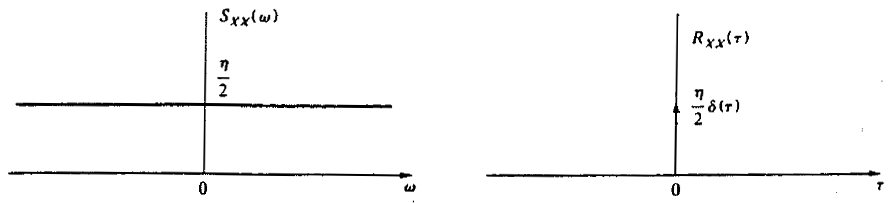
\includegraphics[width=9cm]{bilder/weisses_rauschen.png}
			\end{minipage}
		\end{center}


		\subsubsection{Colored Noise Signals}
		\renewcommand{\arraystretch}{2}
		\begin{tabular}[c]{ | p{4cm} | p{3.5cm} | p{3cm} | p{6cm} | }
			\hline
				\textbf{Term (German)}
				& \textbf{Term (English)}
				& \textbf{Power Spectrum}
				& \textbf{Note} \\
			\hline
				Rosa Rauschen
				& Pink Noise
				& $P_{xx}(\omega) = c \cdot \dfrac{1}{\omega}$
				& Test signal for audio engineering, due to constant power per octave \\
			\hline
				Braunes/Rotes Rauschen
				& Brown/Red Noise
				&   $P_{xx}(\omega) = c \cdot \dfrac{1}{\omega^2}$
				& \\
			\hline
				Blaues Rauschen
				& Blue Noise
				&   $P_{xx}(\omega) = c \cdot \omega$
				& \\
			\hline
				Violettes Rauschen
				& Purple/Violet Noise
				&   $P_{xx}(\omega) = c \cdot \omega^2$
				& \\
			\hline
		\end{tabular}
		\renewcommand{\arraystretch}{1}


\subsection{Estimation \hayes{72}}
  \subsubsection{Bias}
    The bias is the difference between the real value $\Theta$ and the estimate $\hat{\Theta}$: 
    $B = \Theta - E(\hat{\Theta}_N)$. When $B=0$, the estimator is \em unbiased\em. When the estimator
    is biased but the bias goes to zero as the number of observations $N$ goes to infinity, then
    the estimator is \em asymptotically unbiased \em ($\lim_{N \rightarrow \infty} E(\hat{\Theta}_N) = \Theta$). 
    If the bias stays $B \neq 0$, the estimator is \em biased\em.
    
  \subsubsection{Consistency}
    If $\lim_{N \rightarrow \infty} Var(\hat{\Theta}_N) = 0$, the estimator is consistent. 
    $\hat{\Theta}_N$ is said to \em converge to $\Theta$ with probability one\em. 
    Here, a \em consistent \em estimator if it is asymptotically unbiased and has a variance that
    goes to zero as $N$ goes to infinity.
     


\vspace{1em}
\begin{minipage}[t]{11cm}
  \vspace{-1.7cm}
  \section{Signal Modeling \hayes{129}}
  %\renewcommand{\arraystretch}{1.0}
  \textbf{Objective: } Calculate the coefficients for a filter whose
  impulse response matches as closely as possible with a given signal ($x[n]$ - with
  length $N$).

      $$ y(n) = \sum\limits_{k=0}^{q} b(k)x(n-k) - \sum\limits_{k=1}^{p} a(k)y(n-k)$$
      $$ H(z) = \dfrac{B(z)}{A(z)} = \dfrac{b_0 + b_1z^{-1} + b_2 z^{-2} + \dots +
      b_q z^{-q}}{1 + a_1z^{-1} + a_2 z^{-2} + \dots + a_p z^{-p}} $$ 

\end{minipage}
\hfill
\begin{minipage}{7.2cm}
	\vspace{3mm}
	\begin{tabular}{| p{1.4cm} | p{2cm} | p{2.2cm} | }
	    \hline
	    \textbf{Method}
	    & exact match
	    & minimal error \\
	    \hline
	    \hline
	    \textbf{LS} 
	    & $[0]$
	    & $[1, N - 1]$\\
	    \hline
	    \textbf{Padé} 
	    & $[0, q + p + 1]$
	    & -\\
	    \hline
	    \textbf{Prony} 
	    & $[0, q]$
	    & $[q + 1, N - 1]$ \\
	    \hline
	    \textbf{Shanks} 
	    & $[0]$
	    & $[1, N - 1]$\\
	    \hline
	\end{tabular}\\
	$q$: number of zeros\\
	$p$: number of poles\\
	$N$: length of signal $x(n)$
\end{minipage}

\subsection{Least Squares Method \hayes{131}}
The coefficients \textbf{A and B} are estimated using the least squares error method.
Since solving the estimation requires a $p+q$ equation system, this method is very rarely applied.\\
\begin{minipage}{8cm}
	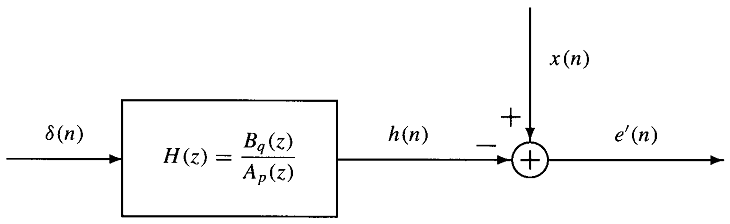
\includegraphics[width=8cm]{../TSM_StatDig/bilder/signalModeling.png}
\end{minipage}
\begin{minipage}{10cm}
$\frac{\partial \sum\limits_{n=0}^{\infty}|e'(n)|^2}{\partial a_p^*(k)}=\frac{1}{2\pi} \int\limits_{-\pi}^{\pi}\left[X(e^{j\omega})-
\frac{B_q(e^{j\omega})}{A_p (e^{j\omega})}\right]\frac{B^*_q(e^{j\omega})}{A_p^* (e^{j\omega})^2}e^{jk\omega} d\omega=0$\\
$\frac{\partial \sum\limits_{n=0}^{\infty}|e'(n)|^2}{\partial b_q^*(k)}=\frac{1}{2\pi} \int\limits_{-\pi}^{\pi}\left[X(e^{j\omega})-
\frac{B_q(e^{j\omega})}{A_p (e^{j\omega})}\right]\frac{e^{jk\omega}}{A_p^* (e^{j\omega})} d\omega=0$\\
\end{minipage} 
\subsubsection{Example FIR Equalizer}
With a FIR first order (2 coefficients) a given sequence (e.g. $[0, 2, 1, 0]$ ) should be filtered so that output is a Dirac $[0, 1 , 0 , 0]$.\\
$\underbrace{\begin{bmatrix}
x[0] 	& 0 	\\
x[1]	& x[0]	\\
0		& x[1]
\end{bmatrix}}_{\bm A}
\cdot \begin{bmatrix}
b_0\\
b_1
\end{bmatrix}=\begin{bmatrix}
1\\
0\\
0
\end{bmatrix}$. To solve the equations the pseudo inverse has to be used: $\bm A^{\dagger} = \left(\bm A^T \cdot \bm A\right)^{-1}\bm A^T 
\Rightarrow \bm  A^\dagger \begin{bmatrix}
1\\
0\\
0
\end{bmatrix}=\begin{bmatrix}
b_0\\
b_1
\end{bmatrix}$

\subsection{Padé Approximation}
The resulting impulse response \textbf{matches exactly} with the given signal $x[n]$ in the interval $[0, q + p + 1]$,
afterwards, the filter is not necessarily stable.

	%\vspace{-0.5cm}
	\renewcommand{\arraystretch}{1.0}
	\begin{aufzaehlung}
  		\item Calculate $a$-coefficients / poles: $\bm X_q \cdot a_p = -x_{q+1} \Longrightarrow a_p = - \bm X_q^{-1} \cdot x_{q+1}$ \matlab{$a_t = - X_t \backslash x$} \small $$
	%	\begin{matrix} n=q+1\\ n=q+2\\ \vdots \\ n=q+p \end{matrix}
		\underbrace{ \begin{bmatrix}
    		x[q]     & x[q-1]   & \hdots & x[q-p+1] \\                                   
    		x[q+1]   & x[q]     & \hdots & x[q-p+2] \\
    		\vdots   & \vdots   & \ddots & \vdots \\                             
    		x[q+p-1] & x[q+p-2] & \hdots & x[q] \\
		\end{bmatrix}  
		}_{\bm  X_q} \cdot 
		\underbrace{\begin{bmatrix}
    		a_1 \\
    		a_2 \\
    		\vdots \\
    		a_p
		\end{bmatrix}  }_{a_p} = \underbrace{\begin{bmatrix}
    		-x [q+1]\\            
    		-x [q+2]\\
    		\vdots \\
    		-x [q+p]\\
		\end{bmatrix}}_{x_{q+1}}  \Longleftrightarrow 
		\begin{bmatrix}
    		x[q+1] & x[q] & \hdots & x[q+1-p] \\                                   
    		x[q+2] & x[q+1] & \hdots & x[q+2-p] \\
    		\vdots & \vdots & \ddots & \vdots \\                             
    		x[q+p] & x[q+p-1] & \hdots & x[q] \\
		\end{bmatrix}
		\begin{bmatrix}
    		1 \\
    		a_1 \\
    		\vdots \\
    		a_p
		\end{bmatrix} = 
		\begin{bmatrix}
    		0 \\
    		0 \\
    		\vdots \\
    		0
		\end{bmatrix} 
		$$  \normalsize
		
		\vspace{-0.5cm}
		If A is singular, the assumption that $a_0 = 1$ was incorrect. $\Longrightarrow$ Set $a_0=0$.
		$ \Longrightarrow \bm X_q \cdot \bm a_p = \bm 0$
		
  		\item Calculate $b$-coefficients / zeros: $\bm X_0 \cdot a_p = b_q$ \small \hspace{0.5cm}
		$ \begin{matrix} n=0\\ n=1\\ \vdots\\ n=q \end{matrix} \overset{(0 \hdots p)}{\underbrace{\begin{bmatrix}
    		x[0] & 0 & \hdots & 0 \\
    		x[1] & x[0] & \hdots & 0 \\
    		\vdots & \vdots & \ddots & \vdots \\
    		x[q] & x[q-1] & \hdots & x[q-p]
		\end{bmatrix}  }_{\bm X_0}}\cdot \underbrace{\begin{bmatrix}
    		1 \\
    		a_1 \\
    		\vdots \\
    		a_p
		\end{bmatrix}  }_{a_p}= 	\underbrace{\begin{bmatrix}
	    		b_0 \\
	    		b_1 \\
	    		\vdots \\
	    		b_q
			\end{bmatrix}}_{b_q}$ \normalsize
			
	\end{aufzaehlung}
	
\vspace{-1.0cm}


\subsection{Prony's Method \hayes{144}}
The resulting impulse response \textbf{matches exactly} with the given signal $x[n]$ in the interval $[0, q]$.
In the interval $[q + 1, N-1]$, the values are approximated with the
\textbf{least squares error} (overdetermined system of equations).


\renewcommand{\arraystretch}{1.0}

\begin{aufzaehlung}
	\item Calculate autocorrelation: $ r_x(k,l) = \sum\limits_{n=q+1}^\infty x(n-l)x^*(n-k)$;\qquad $k,l\geq 0$
	\item Calculate $a$-coefficients: $\bm R_x \cdot a_p = -r_x \Longrightarrow a_p = - \bm R_x^{-1} \cdot r_x$ 
  		\matlab{$a_p = - R_x \backslash r_x$} \small\\
		The minimal error is: $\epsilon_{p,q} = r_x(0,0) + \sum\limits_{k=1}^p a_p(k) r_x(0,k)$
			$$
		\underbrace{\begin{bmatrix}
    		r_x[1,1] & r_x[1,2] & \hdots & r_x[1,p] \\
    		r_x[2,1] & r_x[2,2] & \hdots & r_x[2,p] \\
    		\vdots & \vdots & \ddots & \vdots \\
    		r_x[p,1] & r_x[p,2] & \hdots & r_x[p,p] \\
		\end{bmatrix}  }_{\bm R_x} \cdot
		\underbrace{\begin{bmatrix}
    		a_1 \\
    		\vdots \\
    		a_p
		\end{bmatrix}  }_{a_p}= -\underbrace{\begin{bmatrix}
    		r_x[1,0] \\
    		\vdots \\
    		r_x[p,0]
		\end{bmatrix}  }_{r_x}
		\Longrightarrow
		\begin{bmatrix}
    		r_x[0,0] & r_x[0,1] & \hdots & r_x[0,p] \\ 
    		----&----&----&----\\
    		r_x[1,0] & r_x[1,1] & \hdots & r_x[1,p] \\                                   
    		r_x[2,0] & r_x[2,1] & \hdots & r_x[2,p] \\
    		\vdots & \vdots & \ddots & \vdots \\                             
    		r_x[p,0] & r_x[p,1] & \hdots & r_x[p,p] \\                        
		\end{bmatrix} \cdot 
		\begin{bmatrix}
    		1 \\
    		a_1 \\
    		\vdots \\
    		a_p
		\end{bmatrix} = \begin{bmatrix}
    		\epsilon_{p,q} \\
    		---\\
    		0 \\
    		\vdots \\
    		0
		\end{bmatrix} $$ 
		For all-pole models, the a-coefficients can be directly calculated from the b system of equations. 
		For this, all $b$-coefficients except for $b_0$ must be set to 0.
	\item Calculate $b$-coefficients as in \textbf{Padé}: $\bm X_0 \cdot a_p = b_q$
		\normalsize
\end{aufzaehlung}
	
\subsection{Shanks' Method \hayes{154}}

The B-coefficients are estimated given the A's in such a way that the resulting impulse response in the interval $[0, N - 1]$ with the
\textbf{least squares error} (overdetermined system of equations) approximates the given
signal $x[n]$. The only improvement would be if the A-coefficients could also include all signal values (Least-square).

\begin{aufzaehlung}
  		\item Calculate $a$-coefficients as in \textbf{Prony}: $a_p = - \bm R_x^{-1} \cdot r_x$ \matlab{$a_p = - R_x \backslash r_x$}  
  		\item Calculate impulse response $g[n]$ of the purely recursive filter ($g[n] = \delta(n)- \sum\limits_{k=1}^p a_p(k)g(n-k)$), 
  		or using inverse z-transform of $H(z)$.
  		\item Calculate autocorrelation:  $r_g(k)=\sum\limits_{n=0}^\infty g(n)g^*(n-k)$; or inverse z-transform of $|H(z)|^2$
  		\item Calculate cross-correlation: $r_{xg}(k)=\sum\limits_{n=0}^\infty x(n)g^*(n-k)$
  		\item Calculate $b$-coefficients (for stationary processes): $b_q = R_g^{-1} \cdot r_{xg}$ \matlab{$b_q = R_g \backslash r_{xg}$}\\
  		for\\

		 $$\begin{matrix}n=0\\ n=1\\ \vdots\\ n=N_{ha}+q\\ \end{matrix}
		\overset{(0 \hdots q)}{\underbrace{\begin{bmatrix}
    		r_g(0) & r_g(1) & \hdots & r_g(q) \\                                            
    		r_g(1) & r_g(0) & \hdots & r_g(q-1) \\         
    		\vdots & \vdots & \ddots & \vdots \\                                      
    		r_g(q) &r_g(q-1) & \hdots & r_g(0) \\    
		\end{bmatrix}  }_{R_g}} \cdot \underbrace{\begin{bmatrix}
    		b_0 \\
    		b_1 \\
    		\vdots \\
    		b_q
		\end{bmatrix}  }_{b_q}= \underbrace{\begin{bmatrix}
    		r_{xg}(0) \\
    		r_{xg}(1) \\
    		\vdots \\
    		r_{xg}(q) \\
		\end{bmatrix}  }_{r_{xg}} $$
\end{aufzaehlung}

\subsection{All-Pole Modeling \hayes{160}}
Corresponds to: \ref{sec:autoregressive_model_method}
\begin{enumerate}
	\item Calculate autocorrelation: $ r_x(k) = \sum\limits_{n=0}^\infty x(n)x^*(n-k)$;\qquad $k\geq 0$
	\item Calculate $a$-coefficients: $\bm R_x \cdot a_p = -r_x \Longrightarrow a_p = - \bm R_x^{-1} \cdot r_x$ 
  		\matlab{$a_p = - R_x \backslash r_x$} \small\\
		The minimal error is: $\epsilon_{p} = r_x(0) + \sum\limits_{k=1}^p a_p(k) r_x^*(k)$
			$$
		\underbrace{\begin{bmatrix}
    		r_x(0) & r_x^*(1) & \hdots & r_x^*(p-1) \\
    		r_x(1) & r_x(0) & \hdots & r_x^*(p-2) \\
    		\vdots & \vdots & \ddots & \vdots \\
    		r_x(p-1) & r_x(p-2) & \hdots & r_x(0) \\
		\end{bmatrix}  }_{\bm R_x} \cdot 
		\underbrace{\begin{bmatrix}
    		a_1 \\
    		\vdots \\
    		a_p
		\end{bmatrix}  }_{a_p}= -\underbrace{\begin{bmatrix}
    		r_x(1) \\
    		\vdots \\
    		r_x(p)
		\end{bmatrix}  }_{r_x}$$ 
	\item $b(0) = \sqrt{\epsilon_p}$ 
\end{enumerate}


\subsection{Linear Prediction \hayes{165} (Exercise 4.13)}

		$$\hat{x}(n+n_0) = - \sum\limits_{k=1}^p a_p(k) x(n-k)$$
		$$
		\underbrace{\begin{bmatrix}
    		r_x[1,1] & r_x[1,2] & \hdots & r_x[1,p] \\                                   
    		r_x[2,1] & r_x[2,2] & \hdots & r_x[2,p] \\
    		\vdots & \vdots & \ddots & \vdots \\                             
    		r_x[p,1] & r_x[p,2] & \hdots & r_x[p,p] \\                        
		\end{bmatrix}  }_{\bm R_x} \cdot 
		\underbrace{\begin{bmatrix}
    		a_1 \\
    		\vdots \\
    		a_p
		\end{bmatrix}  }_{a_p}= \underbrace{\begin{bmatrix}
    		r_x[1,-n_0] \\
    		\vdots \\
    		r_x[p,-n_0]
		\end{bmatrix}  }_{r_x}$$

\subsection{FIR Inverse Filter \hayes{166}}
$$G(z)H(z) \approx 1\qquad g(n)*h(n) \approx \delta(n) \qquad r_g(k) = \sum\limits_{n=0}^\infty g(n)g^*(n-k) \qquad \text{Delay: } n_0$$

		$$
		\underbrace{\begin{bmatrix}
    		r_g(0) & r_g(1) & \hdots & r_g(N-1) \\                                   
    		r_g(1) & r_g(0) & \hdots & r_g(N-2) \\
    		\vdots & \vdots & \ddots & \vdots \\                             
    		r_g(N-1) & r_g(N-2) & \hdots & r_g(0) \\                        
		\end{bmatrix}  }_{\bm R_g} \cdot 
		\underbrace{\begin{bmatrix}
    		h_N(0) \\
    		\vdots \\
    		h_N(N-1)
		\end{bmatrix}  }_{h_N}= -\underbrace{\begin{bmatrix}
    		g(n_0) \\
    		g(n_0 - 1)	 \\
    		\vdots \\
    		g(0)\\
    		0\\
    		\vdots \\
    		0
		\end{bmatrix}  }_{r_{gd}}$$


		\subsection{Approximation with limited data using All-Pole Filter}
		\subsubsection{Autocorrelation Method \hayes{178}}
		Given the autocorrelations, see Chapter \ref{sec:autoregressive_model_method}.\\
		Assumption: The data $x[n]$ is zero outside the definition range ($n=[0..N]$): $x[n]=0$. This forces the filter into a stable state.
		\renewcommand{\arraystretch}{1.0}
		
		\begin{enumerate}
			\item Calculate $a$-coefficients (using Pseudoinverse / generalized Inverse): $a_p = -\left(\bm X_p^T \cdot \bm  X_p\right)^{-1} \cdot \bm X_p^T \cdot x_1$
				  \matlab{$a_p = -X_p \backslash x_1$} \small
					$$
				\begin{matrix} n=q+1\\ n=q+2\\ \vdots \\ n=N\\ n=N+1\\ \vdots \\ N+p
				\end{matrix}
				\underbrace{\begin{bmatrix}
					x[0] & 0 & \hdots & 0 \\ 
					x[1] & x[0] & \hdots & 0 \\ 
					x[2] & x[1] & \hdots & 0 \\        
					\vdots & \vdots & \ddots & \vdots \\
					----&----&----&----\\                
					x[p-1] & x[p-2] & \hdots & x[0] \\                                   
					x[p] & x[p-1] & \hdots & x[1] \\      
					\vdots & \vdots & \ddots & \vdots \\                        
					x[N-1] & x[N-2] & \hdots & x[N-p] \\ 
					----&----&----&----\\                            
					x[N] & x[N-1] & \hdots & x[N-p+1] \\ 
					0 & x[N] & \hdots & x[N+2-p] \\
					\vdots & \vdots & \ddots & \vdots \\                     
					0 & 0 & \hdots & x[N] \\
				\end{bmatrix}  }_{\bm X_p=(N+p \; \times \; p) Matrix} \cdot \underbrace{\begin{bmatrix}
					a_1 \\
					\vdots \\
					a_p
				\end{bmatrix}  }_{a_p}= \underbrace{\begin{bmatrix}
					 -x [1]\\            
					 -x [2]\\
					\vdots \\
					 -x [N]\\
					0 \\
					\vdots \\
					0
				\end{bmatrix}}_{x_1} 
				 $$ \normalsize
			\end{enumerate}
			
		\subsubsection{Covariance Method  \hayes{183}}
		No assumptions are made, only the existing data is used. A disadvantage is that the filter can become unstable. 
		Another disadvantage is that A is not a Toeplitz matrix, so solving it is not as straightforward as with the Autocorrelation Method. 
		However, the signal is reconstructed more accurately. For a data series corresponding to an impulse response, the filter is perfectly reconstructed. 
		With the disadvantage that unstable poles are also implemented. $a_p = -\left(\bm X_p^T \cdot \bm  X_p\right)^{-1} \cdot \bm X_p^T \cdot x_p$ \matlab{$a_p = -X_p \backslash x_p$} \small
				$$
				\underbrace{\begin{bmatrix}               
					x[p-1] & x[p-2] & \hdots & x[0] \\                                   
					x[p] & x[p-1] & \hdots & x[1] \\      
					\vdots & \vdots & \ddots & \vdots \\                        
					x[N-1] & x[N-2] & \hdots & x[N-p] \\ 
				\end{bmatrix}  }_{\bm X_p} \cdot \underbrace{\begin{bmatrix}
					a_1 \\
					\vdots \\
					a_p
				\end{bmatrix}  }_{a_p}= \underbrace{\begin{bmatrix}
					 -x[p]\\            
					 -x[p+1]\\
					\vdots \\
					 -x[N]\\
				\end{bmatrix}}_{x_p}
				 $$ \normalsize
		(Note: These equations are a subset of the equations of the Autocorrelation Method.)


\subsection{Stochastic Models}
In stochastic models, generally the same models are used as in the deterministic world.
Instead of the Dirac pulse, white noise is used at the input of the filter, and the autocorrelation is formed using the expected value.
$r_x(k)=E\{x(n) \cdot x^*(n-k)\}$\\
Instead of the cross-correlation $r_{gx}$, the convolution of $b_q(k)$ and $h^*(-k)$ is used.\\
$c_q(k) = b_q(k) \ast h^*(-k) = \sum_{l=0}^{q-k} b_q(l+k) h^*(l)$

\subsubsection{Autoregressive Moving Average Models, ARMA \hayes{189}}
An ARMA(p,q) process is white noise that is filtered through an LTI system $H(z)$.\\
To determine the coefficients of $H(z)=\frac{B_q(z)}{A_p(z)}=\frac{\sum\limits_{k=0}^q b_q(k)z^{-k}}{1+\sum\limits_{k=1}^p a_p(k)z^{-k}}$, the \textbf{extended Yule-Walker equations} are solved:
\small$$
\underbrace{\begin{bmatrix}               
			r_x[0] & r_x^*[1] & \hdots & r_x^*[p] \\   
			r_x[1] & r_x[0] & \hdots & r_x^*[p-1] \\   
			\vdots & \vdots & \ddots & \vdots \\     
			r_x[q] & r_x[q-1] & \hdots & r_x[q-p] \\   
			r_x[q+1] & r_x[q] & \hdots & r_x[q-p+1] \\    
			\vdots & \vdots & \ddots & \vdots \\     
			r_x[L] & r_x[L-1] & \hdots & r_x[L-p] \\ 
		\end{bmatrix}  }_{R_x} \cdot \underbrace{\begin{bmatrix}
			1\\
			a_p(1) \\
			a_p(2) \\
			\vdots \\
			a_p(p)
		\end{bmatrix}  }_{a_p}= \begin{bmatrix}
				c_q[0]\\            
				c_q[1]\\
			\vdots \\
				c_q[q]\\
				0\\
			\vdots \\
				0\\
		\end{bmatrix} 
			$$ \normalsize

\begin{aufzaehlung}
			\item Calculate the A- coefficients: $R_q \cdot a_p = - r_{q+1}$
			\small$$
\underbrace{\begin{bmatrix}                   
			r_x[q] & r_x[q-1] & \hdots & r_x[q-p+1] \\   
			r_x[q+1] & r_x[q] & \hdots & r_x[q-p+2] \\    
			\vdots & \vdots & \ddots & \vdots \\     
			r_x[q+p-1] & r_x[q+p-2] & \hdots & r_x[q] \\ 
		\end{bmatrix}  }_{R_q} \cdot \underbrace{\begin{bmatrix}
			a_p(1) \\
			a_p(2) \\
			\vdots \\
			a_p(p)
		\end{bmatrix}  }_{a_p}= \underbrace{\begin{bmatrix}
				-r_x[q+1]\\            
				-r_x[q+2]\\
			\vdots \\
				-r_x[q+p]\\
		\end{bmatrix}}_{r_{q+1}} 
			$$ \normalsize
			\item To calculate the B- coefficients, one must go via the C- coefficients: $R_x \cdot a_p = c_q$
	
			\small$$
\underbrace{\begin{bmatrix}                   
			r_x[0] & r_x^*[1] & \hdots & r_x^*[p] \\   
			r_x[1] & r_x[0] & \hdots & r_x^*[p-1] \\    
			\vdots & \vdots & \ddots & \vdots \\     
			r_x[q] & r_x[q+1] & \hdots & r_x[0] \\ 
		\end{bmatrix}  }_{R_x} \cdot \underbrace{\begin{bmatrix}
			1 \\
			a_p(1) \\
			a_p(2) \\
			\vdots \\
			a_p(p)
		\end{bmatrix}  }_{a_p}= \underbrace{\begin{bmatrix}
				c_q[0]\\            
				c_q[1]\\
			\vdots \\
				c_q[q]\\
		\end{bmatrix}}_{c_{q}} 
			$$ \normalsize	 
			\item Write down $[C_q(z)]_+$: $[C_q(z)]_+ = \sum\limits_{k=0}^q c_q(k)z^{-k}$
			\item Calculate $[P_y(z)]_+=\left[[C_q(z)]_+ \cdot A^*_p(1/z^*)\right]_+$ e.g. $[C_1(z)]_+=\frac{45}{2}-6z^{-1}$, $A^*_p(1/z^*)=1-0.5z$; $[C_1(z)]_+ \cdot A^*_p(1/z^*)= -\frac{45}{4}z +\frac{51}{2}-6z^{-1}$ $\Rightarrow$  $[P_y(z)]_+= \frac{51}{2}-6z^{-1}$
			\item Make $[P_y(z)]_+$ symmetric. e.g.: $P_y(z) =  -6 z +\frac{51}{2}-6z^{-1}$
			\item Factorize $P_y(z)=B_q(z)B_q^*(1/z^*)$ so $B_p(z)$ can be used: \\
			e.g. $B_1(z)\cdot B_1^*(1/z^*)= \underbrace{2\sqrt{6}(1-\frac{1}{4}z^{-1})}_{B_q(z)}\cdot \underbrace{2\sqrt{6}(1-\frac{1}{4}z^{1})}_{B_q^*(1/z^*)}$
			\item $H(z)=\frac{B_q(z)}{A_p(z)}$ e.g.: $H(z)=\frac{2 \sqrt{6}(1-\frac 1 4 z^{-1})}{A_p(z)}$
\end{aufzaehlung}


\subsubsection{Autoregressive Models - AR \hayes{194}}
\label{sec:autoregressive_model_method}
In the AR(p) model, the ARMA(p,q=0) method is used, but only with poles. $H(z)=\frac{b(0)}{1+\sum\limits_{k=1}^{p} a_p(k)z^{-k}}$.\\
 $$\begin{bmatrix} 
	 	r_x(0)  & r_x^*(1) & r_x^*(2) & \cdots & r_x^*(p-1)\\
	 	r_x(1)  & r_x(0) & r_x^*(1) & \cdots & r_x^*(p-2)\\
	 	r_x(2)  & r_x(1) & r_x(0) & \cdots & r_x^*(p-3)\\
	 	\vdots  & \vdots  & \vdots  & \ddots & \vdots\\
	 	r_x(p-1)& r_x(p-2)& r_x(p-3)& \cdots &  r_x(0)\\
   \end{bmatrix} \cdot
   \begin{bmatrix}
    	a_p(1)\\
    	a_p(2)\\
    	a_p(3)\\
    	\vdots\\
    	a_p(p)\\
   \end{bmatrix}=
   \begin{bmatrix}
       	-r_x(1)\\
       	-r_x(2)\\
       	-r_x(3)\\
       	\vdots\\
        -r_x(p)\\
   \end{bmatrix}
 $$
 With $|b(0)|^2=r_x(0) + \sum\limits_{k=1}^{p} a_p(k)r_x(k)$
 

 
 \subsubsection{Moving Average Models - MA \hayes{195}}
A MA process is a special form of an ARMA(p=0,q) process, which only has zeros.\\
$P_x(z)=\sum\limits_{k=-q}^{q}r_x(k)z^{-k}=B_q(z)B_q^*(1/z^*)$
\begin{aufzaehlung}
	\item Spectrally factorize $P_x(z)$ into: $P_x(z)=\sigma^2_0 \cdot Q(z)\cdot Q^*(1/z^*)=\underbrace{\sigma^2_0}_{|b_q(0)|^2} \underbrace{\prod\limits_{k=1}^q (1-\beta_k z^{-1})}_{B_q(z)} \cdot \underbrace{\prod\limits_{k=1}^q (1-\beta_k^* z)}_{B^*_q(1/z^*)}$
	\item Expand $B_q(z)$ $\Rightarrow$ minimum phase filter (all zeros are inside the unit circle)
	\item Or, expand $B_q^*(1/z^*)$ to get a maximum phase filter (all zeros are outside the unit circle)
\end{aufzaehlung}


\section{Optimum Filters}
An optimum filter minimizes the mean-square error $\xi = E\left(|e(n)|^2\right) \quad x(n)=d(n)+v(n) \quad e(n) = d(n) - \tilde{d}(n)$\\
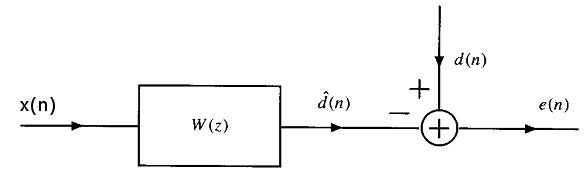
\includegraphics[width=9cm]{../TSM_StatDig/bilder/optimumFilter.jpg}\\
The minimal error is \textbf{always orthogonal} to the data: $E{e(n)x^*(n-k)}=0$ $\forall$ $k\in[0,p-1]$

\subsection{Wiener FIR Filter \hayes{337}}
\begin{minipage}{10cm}
\begin{tabbing}

Wiener-Hopf equations: \= $\sum \limits_{l=0}^{p-1} w(l)r_x(k-l)=r_{dx}(k)$; $\forall$ $k\in[0,p-1]$ \\
Correlations:  \>
						$r_x(k)=E \{ x(n)x^{*}(n-k) \}$ \\
\>						$r_{dx}(k)=E\{d(n)x^{*}(n-k)\}$ \\
Minimum Error: \>		$\xi_{min}=r_d(0)-\sum \limits_{l=0}^l w(l)r_{dx}^{*}(l)$
\end{tabbing}
\end{minipage}
\begin{minipage}{10cm}
$\small
\underbrace{\begin{bmatrix}                   
    		r_x[0] & r_x^*[1] & \hdots & r_x^*[p-1] \\   
    		r_x[1] & r_x[0] & \hdots & r_x^*[p-2] \\    
    		\vdots & \vdots & \ddots & \vdots \\     
    		r_x[p-1] & r_x[p-2] & \hdots & r_x[0] \\ 
		\end{bmatrix}  }_{R_x} \cdot \underbrace{\begin{bmatrix}
    		w(0) \\
    		w(1) \\
    		\vdots \\
    		w(p-1)
		\end{bmatrix}  }_{w}= \underbrace{\begin{bmatrix}
    		 r_{dx}[0]\\            
    		 r_{dx}[1]\\
    		\vdots \\
    		 r_{dx}[p-1]\\
		\end{bmatrix}}_{r_{dx}} 
		 $$ \normalsize	 $\\
$$R_x \cdot w =r_{dx}$$
\end{minipage}
\begin{minipage}{7.5cm}
\subsubsection{Filtering \hayes{339}}
The input signal is $x(n)=d(n)+v(n)$. Because the noise and data signals are uncorrollated and the noise has zero mean, the Wiener-Hopf equation simplifies as follows:\\
$r_x(k)=r_d(k)+r_v(k)$\\
$r_{dx}(k)=r_d(k) \hspace{1.5cm} \rightarrow [R_d + R_v]\cdot w = r_d$\\
 with $R_v=\small \begin{bmatrix}                   
    		\sigma_v^2 & \hdots & 0\\   
    		\vdots & \ddots & \vdots \\     
    		0&  \hdots &\sigma_v^2 \\ 
		\end{bmatrix} $
\end{minipage}
\hspace{3mm}
\begin{minipage}{10.8cm}
\subsubsection{Linear Prediction FIR \hayes{342}}
$\hat{x}(n+\alpha)=\sum \limits_{k=0}^{p-1} w(k)[x(n-k)+v(n-k)]$

$ 	\hookrightarrow  	\small \begin{bmatrix}                   
    		r_y[0] & r_y^*[1] & \hdots & r_y^*[p-1] \\   
    		r_y[1] & r_y[0] & \hdots & r_y^*[p-2] \\    
    		\vdots & \vdots & \ddots & \vdots \\     
    		r_y[p-1] & r_y[p-2] & \hdots & r_y[0] \\  
		\end{bmatrix}   \cdot \begin{bmatrix}
    		w(0) \\
    		w(1) \\
    		\vdots \\
    		w(p-1)
		\end{bmatrix} = \begin{bmatrix}
    		 r_{x}[\alpha]\\            
    		 r_{x}[\alpha+1]\\
    		\vdots \\
    		 r_{x}[\alpha+p-1]\\
		\end{bmatrix}
$$ \normalsize	 $\\
$\alpha$ are the steps to predict. Noise: $r_y(k) = r_x(k) + r_v(k)$\\
\end{minipage}\\
\begin{minipage}{11.5cm}
\subsubsection{Linear Phase Filter \hayes{17}, exercise 9.16} 
All frequency are delayed same. \\
For \textbf{FIR}: the coefficients are symmetric $(w_n(0)z^1+w_n(1)z^0+w_n(0)z^{-1})$ or with a causal filter: $w_n(0)z^0 + w_n(1)z^{-1} + w_n(0)z^{-2}$\\
$\small \begin{bmatrix}
2 r_x[0] + 2 r_x[2]		&	2 r_x[1] \\
2 r_x[1]				& 	r_x[0]
\end{bmatrix} \cdot \begin{bmatrix}
w_n(0)\\
w_n(1)
\end{bmatrix}= \underbrace{ \begin{bmatrix}
r_x[\alpha] + r_x[\alpha+2]\\
r_x[\alpha+1]
\end{bmatrix}}_{\text{for linear prediction} } 
= \underbrace{ \begin{bmatrix} = 
r_{dx}[0] + r_{dx}[2]\\
r_{dx}[1]
\end{bmatrix}    }_{\text{for optimal filter} }  $

\end{minipage}
\hspace{3mm}
\begin{minipage}{7cm}
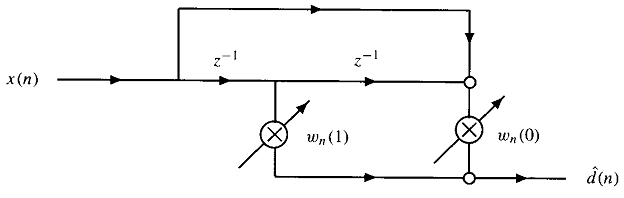
\includegraphics[width=7cm]{../TSM_StatDig/bilder/linear_phase_fir.png}
How a linear phase FIR filter 2 order is implemented in hardware.
\end{minipage}
\subsection{Wiener IIR Filter}
\begin{minipage}{8cm}
\subsubsection{Noncausal \hayes{353}}
\begin{tabbing}
Wiener-Hopf equations: \=
$H(e^{jw})=\frac{P_{dx}(e^{jw})}{P_{x}(e^{jw})}  \Rightarrow
\frac{P_{d}(e^{jw})}{P_{d}(e^{jw}) + P_{v}(e^{jw})}= \frac{SNR(e^{j\omega})}{SNR(e^{j\omega}) + 1}$ (often called \textbf{the} Wiener Filter) \\

Correlations: \>
	$r_x(k) =E \{ x(n)x^{*}(n-k) \} $\\ 
	\>$r_{dx}(k) =E\{d(n)x^{*}(n-k)\}$\\


Minimum Error:\>
	$\xi_{min} =r_d(0)-\sum \limits_{l=-\infty}^\infty h(l)r_{dx}^{*}(l)
	=\frac{1}{2\pi}\int \limits_{-\pi}^\pi[P_d(e^{jw})-H(e^{jw})P_{dx}^{*}(e^{jw})]dw$\\
	\>$=r_d(0)-\frac{1}{2\pi}\int \limits_{-\pi}^\pi[H(e^{jw})P_{dx}^{*}(e^{jw})]dw$
\end{tabbing}

\end{minipage}

\subsubsection{Causal \hayes{358}}
\begin{tabbing}
Spectral Factorization: \=
$ P_x(z) = \sigma_0^2 Q(z) Q^*(z^{-1}) $\\

System function:\hspace{1.2cm}\>
	$H(z)=\frac{1}{\sigma_0^2 Q(z) } [\frac{P_{dx}(z)}{Q^*(z^{-1})} ]_+ $ \\
	
Minimum Error:\>$\xi_{min} =r_d(0)-\sum \limits_{l=0}^\infty h(l)r_{dx}^{*}(l)
	=\frac{1}{2\pi}\int \limits_{-\pi}^\pi[P_d(e^{jw})-H(e^{jw})P_{dx}^{*}(e^{jw})]dw$\\
	
\end{tabbing}
Example \hayes{362}

\subsubsection{Linear Prediction IIR \hayes{365}}
\begin{tabbing}
System function:\hspace{0.2cm}\=
	$ r_{dx}(k)=r_x(k+\alpha)  \qquad \alpha \text{ = steps to predict.} $\\
\>	$ H(z)= \frac{1}{Q(z)}[z^\alpha Q(z)]_+ $ \hspace{6.8cm} \=$\rightarrow \text{monic, one step } H(z) = z [1- \frac{1}{Q(z)}] $\\
Minimum Error:\>
	$\xi_{min} =r_d(0)-\sum \limits_{l=0}^\infty h(l)r_{dx}^{*}(l)
		=\frac{1}{2\pi}\int \limits_{-\pi}^\pi[P_d(e^{jw})-H(e^{jw})P_{dx}^{*}(e^{jw})]dw $\>$ \rightarrow \text{monic, one step } \xi_{min} = \sigma^2_0$\\
\end{tabbing}


\subsubsection{Wiener Deconvolution \hayes{369}}
Deconvolutate a signal $x(n)=d(n)\ast g(n) + w(n)$ (not $x(n)=d(n) + g(n)$) it's not easy. At the best, the signal could be reconstruct as:
$\hat{D}(e^{\omega})=D(e^{j\omega}) + \frac{W(e^{j\omega})}{G(e^{j\omega})}=D(e^{j\omega})+V(e^{j\omega})$ \quad $V(e^{j\omega})$ isn't anymore white noise. 
Espacialy if $G(e^{j\omega})$ becomes small the noise will be amplified.\\
System function:\hspace{1.2cm}
	$ H(z)= \frac{1}{G(z)}\left[\frac{P_d(z)}{P_d(z)+P_w(z)/|G(z)|^2}\right]$\\


\subsection{Discrete Kalman Filter}
The Kalman Filter is a Best Linear Unbiased Estimator (BLUE).

\textbf{Basic Idea} The Kalman Filter estimates the Kalman Gain based on
the least squares error. Specifically, the Kalman Filter defines measurement values
using state variables and a noise signal. \\
\subsubsection{Prerequisites}
\begin{itemize}
	\item A physical model/system development (for the standard version, even a
	linear model)
	\item Measurement values, sensor fusion possible (multiple measurements for one
	system state)
	\item For standard Kalman: linear relationship between measurement values and
	state variables
\end{itemize}
\begin{minipage}{8cm}
	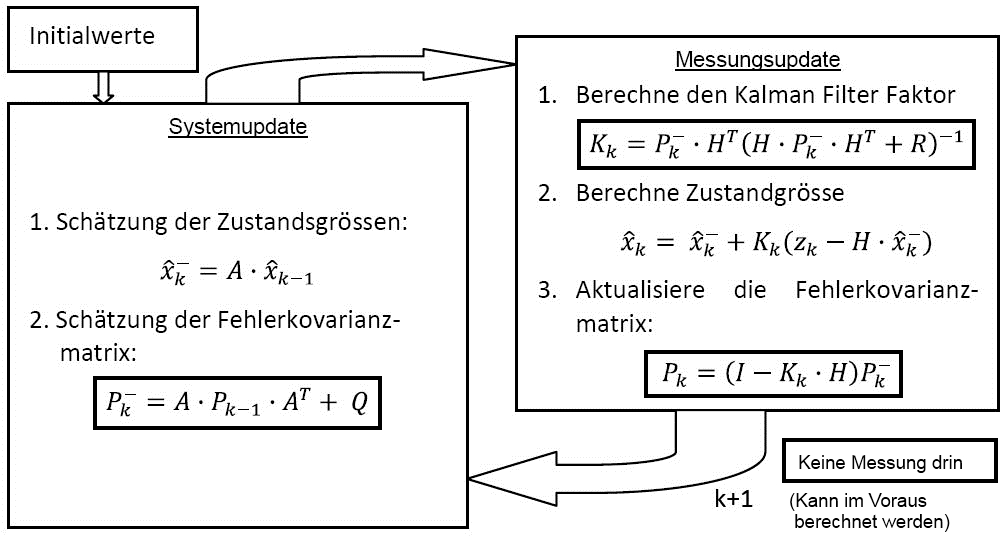
\includegraphics[width=8cm]{Content/AdaptSigVer/KalmanFilter.jpg}
	
	\begin{itemize}
		\item $\hat{x}_{k-1}$ and $P_{k-1}$ require initialization values
		\item $P_K$ and $K_K$ can be pre-calculated offline if the system does not change
	\end{itemize}
	
\end{minipage}
\begin{minipage}{11cm}
	\small
	\subsubsection{Function}
		\begin{itemize}
			\item A System development matrix: Physical model
			\item K Kalman Gain: Weights internal estimation and the measurements of
			individual sensors (0=Only internal estimation;1=only measurement)
			\item H Measurement matrix: Relationship between measurement and state variables
			\item P (Error covariance matrix) Estimate of the error. The larger it is, the
			more the current measurement is considered. In the normal Kalman Filter,
			this converges over time.
			\item z: Measurement values (also from several similar sensors possible)
			\item x: State variables
			\item Initial value: System values arbitrary; Error covariance matrix chosen very
			large, so that initially only the measurement is considered
			\item Q Standard deviation of the system (system noise)
			\item R Standard deviation of the sensors (measurement noise)
			\item The ratio of Q to R is responsible for the filter setting.\newline
			$\frac QR$ large $\rightarrow$ trusts the measurement data more\newline \hspace{4cm} $\frac QR$ small $\rightarrow$ trusts the system properties more
		\end{itemize}
	\normalsize
\end{minipage}



\subsubsection{Kalman Algorithm}
Idea: Best estimation when process and observer equation as well as some initial conditions are given.
$\mathbf{\hat x}(n|n)$ is the prediction, $\mathbf{P}$ is the error covariance matrix, $\mathbf{K}$ is the Kalman gain.
The index $\mathbf{\hat x}(a|b)$ $a$ stands for the iteration number ($n$ = now) and $b$ is which input
data has to be taken ($n-1$ = data up to the last iteration). 
\begin{alignat}{2}
    &\text{State equation:}\qquad&&\mathbf{x}(n) =\mathbf{A}(n-1)\mathbf{x}(n-1) + \mathbf{w}(n) \qquad 
     \mathbf{Q}_w = \text{noise covariance matrix} \underbrace{= \sigma_w^2}_{\text{when one dimensional}}  \nonumber\\
    &\text{Observer equation:}\qquad&&\mathbf{y}(n) =\mathbf{C}(n)\mathbf{x}(n) + \mathbf{v}(n) \qquad \qquad \quad \quad
   \mathbf{Q}_V = \text{noise covariance matrix} \underbrace{= \sigma_v^2}_{\text{when one dimensional}} \nonumber\\
    \nonumber\\
    &\text{Initial condition:}    \qquad    &&\mathbf{x}(0|0)=E\{\mathbf{x}(0)\} \qquad \qquad \text{might be zero}\nonumber\\
                                        &&&\mathbf{P}(0|0)=E\{\mathbf{x}(0)\mathbf{x}^{\mathrm T}(0)\} \qquad \text{should be high}\nonumber\\
    \nonumber\\
    &\text{Prediction:}            \qquad    &&\mathbf{\hat{x}}(n|n-1)=\mathbf{A}(n-1)\mathbf{\hat{x}}(n-1|n-1)\\
                                        &&&\mathbf{P}(n|n-1)=\mathbf{A}(n-1)\mathbf{P}(n-1|n-1)\mathbf{A}^{\mathrm T}(n-1) + \mathbf{Q}_w(n)\\
    \nonumber\\
    &\text{Update:}                \qquad    &&\mathbf{K}(n)=\mathbf{P}(n|n-1)\mathbf{C}^{\mathrm T}(n)\left[\mathbf{C}(n) \mathbf{P}(n|n-1)\mathbf{C}^{\mathrm T}(n)+\mathbf{Q}_v(n)\right]^{-1}\\
                                        &&&\mathbf{\hat{x}}(n|n)=\mathbf{\hat{x}}(n|n-1)+\mathbf{K}(n)\left[\mathbf{y}(n)-\mathbf{C}(n)\mathbf{\hat{x}}(n|n-1)\right]\\
                                        &&&\mathbf{P}(n|n)=\left[\mathbf{I}-\mathbf{K}(n)\mathbf{C}(n)\right]\mathbf{P}(n|n-1)\\
                                        &&&\text{continue with prediction step}    
\end{alignat}


The steady-state is reached when $\mathbf{P}(n|n) = \mathbf{P}(n-1 | n-1)$ and $\mathbf{K}(n) = \mathbf{P}(n|n)$.

\subsubsection{Simplified Principle of the Kalman Filter}
\begin{minipage}{14.5cm}
Given two inaccurate sensors $T_1$ and $T_2$ (uncorrelated), measuring the same signal with known standard deviations $\sigma_1$ and $\sigma_2$. The best
estimator $\hat{T}$ is calculated as follows:\\
\end{minipage}
\hspace{0.25cm}
\begin{minipage}{5cm}
$\hat{T}=\frac{\sigma_1^2}{\sigma_1^2+\sigma_2^2}\cdot T_2+\frac{\sigma_2^2}{\sigma_1^2+\sigma_2^2}\cdot T_1$
\end{minipage}
\begin{minipage}{14.5cm}
Given two correlated signals $T_1$ and $T_2$ with known $\sigma_1$, $\sigma_2$, and the correlation coefficient $\rho$. The best
estimator $\hat{T}$ is calculated as follows:\\
\end{minipage}
\hspace{0.25cm}
\begin{minipage}{5cm}
$\hat{T}=k_1\cdot T_1 + k_2\cdot T_2$\\
$k_1=\frac{\sigma_2^2-\rho \sigma_1 \sigma_2}{\sigma_1^2 - 2 \rho \sigma_1 \sigma_2 + \sigma_2^2}$\\
$k_2=1-k_1=\frac{\sigma_1^2-\rho \sigma_1 \sigma_2}{\sigma_1^2 - 2 \rho \sigma_1 \sigma_2 + \sigma_2^2}$\\
\end{minipage}


\subsubsection{Kalman Modelling of Known System Behaviour}
When a system has known behaviour, the state space representation can be used to find the Kalman matrices. The system is interpreted as a measurement with input $w(n)$ (measurement noise), output $y(n)$ and an added process noise $v(n)$ that is directly added to $y(n)$. 

\begin{longtable}[H]{|>{\bfseries}p{0.3\textwidth}|p{0.65\textwidth}|}
	\hline
	1.: General transfer function:
		& $H(z) = \dfrac{Y(z)}{W(z)} = \dfrac{b_0 + b_1z^{-1} + b_2 z^{-2} + \dots + b_q z^{-q}}{1 + a_1z^{-1} + a_2 z^{-2} + \dots + a_p z^{-p}}$\\
		& \color{red}{Warning: The z-Transform of a known model does not always yield the correct difference equation! For example if a pole is on the unit circle\newline e.g $y(n) = (-1)^n \FT \frac{1}{1+z^{-1}} \IFT y(n) \neq 1 - y(n-1)$.\newline \textrightarrow What you need to do is to find the difference equation! The z-Transform might be one way to do that, but it doesn't always work.}\\
	\hline
	2.: Difference equation:
		& $y(n) = v(n) + b_0 w(n) + \ldots + b_q w(n-q) - a_1y(n-1) + \ldots - a_q y(n-q)$\\
	\hline
	3.: States:
		& {\begin{align*}
				x(n) 	&= w(n) - a_1 x(n-1) - a_2 x(n-2) - \ldots - a_p x(n-p)\\
				x(n-1)	&= x(n-1)\\
				\vdots 	&=	\vdots\\
				x(n-max(p,q) &= x(n-max(p,q))\\
		\end{align*}}\\
		& For more information see \href{https://github.com/HSR-Stud/DigSig2}{DigSig2 cheat sheet section 1.2 Canonical Form}. (Flow diagram and states)\\
	\hline
	4.: State space representation:
		& $A = \begin{bmatrix}
			-a_1 	& -a_2 		& \dots 	& -a_{p-1}	& -a_p\\
			1		& 0			& \dots		& 0			& 0\\
			0		& 1			& \dots		& 			& 0\\
			\vdots	& \vdots	& \ddots	& \vdots	& 0\\
			0		& 0			& \dots		& 1			& 0\\	
		\end{bmatrix}, 
		B = \begin{bmatrix}
			w(n)\\
			0\\
			0\\
			\vdots\\
			0\\
		\end{bmatrix}$\\
		& $C = \begin{bmatrix}
			b_0 & b_1 & \dots & b_q\
		\end{bmatrix}, D = v(n)$\\
	\hline
\end{longtable}


\section{Spectrum Estimation}
The problem of estimation a spectrum is, that there is never an infinity number of samples.
Therefore, the autocorrelation is always multiplied with a window.

\subsection{Nonparametric Method - Periodogram \hayes{393}}
\begin{tabbing}
autocorrelation: 	\= $\hat{r}_x(k) =\frac{1}{N} \sum \limits_{n=0}^{N-1-k} x(n+k)x^*(n)$   \hspace{4cm} \= $k=0,1,\ldots,N-1$ \\
power spectrum:  	\>  $\hat{P}_{per}(e^{jw}) = \frac{1}{N} X_N(e^{jw})X^*_N(e^{jw}) = $\\
\>					$\frac{1}{N}  \left\lvert X_N(e^{jw}) \right\rvert ^2 =  \frac{1}{N}  \left\lvert \sum\limits_{n=0}^{N-1} x(n)e^{-jn\omega} \right\rvert ^2$   \\
computing:  		\> The easiest way to compute the Periodogram is to compute the FFT, take the absolute values and square it\\
					\> $x_N(n) \xrightarrow{DFT} X_N(e^{jw}) \Rightarrow \frac{1}{N}  \left\lvert X_N(k) \right\rvert ^2 = \hat{P}_{per}(e^{j 2 \pi k/N})$ \\
Bias: 				\>  $E\left\lbrace \hat{P}_{per}(e^{jw}) \right\rbrace = \frac{1}{2 \pi}P_x(e^{jw})*W_B(e^{jw})$ \> $W_B$ $\to$ Bartlet window\\
Resolution: 		\>  $Res[\hat{P}_{per}(e^{jw})] = \Delta w = 0.89 \frac{2 \pi}{N}$\> Resolution = 3dB BW $(\Delta\omega)_{3dB}$\\
The Problem of the Periodogram is that the variance doesn't get smaller and it's far \textbf{too big!!!}.\\
Variance 			\> $Var\left\lbrace \hat{P}_{per}^{(i)}(e^{j\omega}) \right\rbrace \approx P^2_x(e^{j\omega})$\\
\end{tabbing}
Because the samples are multiplied with a rectangle window, a dirac in the original power spectrum becomes a sinc with a first sidelobe just 13 dB lower than the mainlobe.\\


The Periodogram is okay to be used when a high frequency resolution is required but should
not be used to estimate the spectrum accurately.

\subsection{Nonparametric Method - Modified Periodogram \hayes{408}}
To have a better sidelobe ratio, different windows are used to multiplied the given data.
\begin{tabbing}
autocorrelation: 	\= $\hat{r}_x(k) =\frac{1}{N} \sum \limits_{n=0}^{N-1-k} x(n+k)x^*(n)$   \hspace{4cm} \= $k=0,1,\ldots,N-1$ \\
power spectrum:  	\>  $\hat{P}_{M}(e^{jw}) = \frac{1}{NU}  \left\lvert \sum\limits_{n=\infty}^{\infty} w(n)x(n)e^{-jn\omega} \right\rvert ^2$   \\
scaling 			\> Because the window itself hasn't normaly a power of 1, the power spectrum has to be scaled by factor U:\\
\>					$U=\frac{1}{N} \sum\limits_{n=0}^{N-1}|w(n)|^2$\\
Bias: 				\>  $E\left\lbrace \hat{P}_{M}(e^{jw}) \right\rbrace = \frac{1}{2 \pi NU}P_x(e^{jw})*|W(e^{jw})|^2$\\
Resolution : 		\>  Window dependent\\
\textbf{The problem of variance isn't solved.}\\
Variance 			\> $Var\left\lbrace \hat{P}_{M}^{(i)}(e^{j\omega}) \right\rbrace \approx P^2_x(e^{j\omega})$\\
\end{tabbing}

\begin{minipage}{10cm}
\begin{tabular}{p{3cm} p{3cm} p{3cm}}
Window	 &  	Sidelobe 	&3dB BW\\
&				Level (dB)	& $(\Delta\omega)_{3dB}$\\
\hline
Rectangular&			-13	&		0.89 (2$\pi$/ N)\\
Bartlett (triangle)&	-27	&		1.28 (2$\pi$/ N)\\
Hann				&	-32	&		1.44 (2$\pi$/ N)\\
Hamming&				-43	&		1.30 (2$\pi$/ N)\\
Backman		&			-58	&		1.68 (2$\pi$/ N)
\end{tabular}
\end{minipage}
\begin{minipage}{8cm}
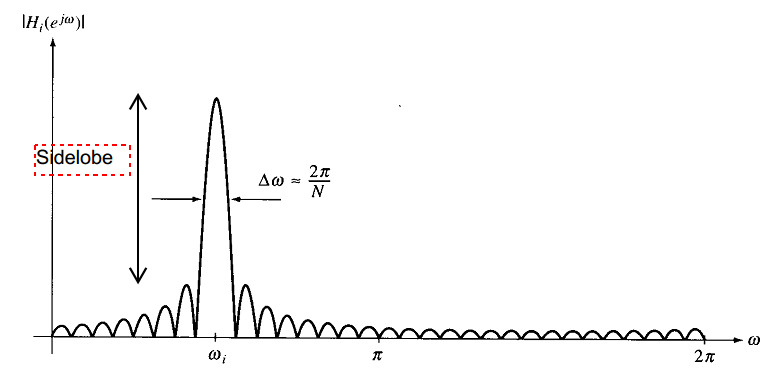
\includegraphics[width=8cm]{./bilder/sidelobe.jpg}
\end{minipage}





\subsection{Nonparametric Method - Bartlett's Method \hayes{412}}
The idea of Bartlett was to take $K$ non-overlapping sub-sequences (lenght $L$) of the given data.
A Periodogram (rectangular window) has to be calculated for every sub-sequence and then averaged. $N=K\cdot L$

\begin{tabbing}
power spectrum:  	\=  $\hat{P}_{B}(e^{jw}) = E\left\{\frac{1}{L}  \left|X_L(e^{jw})\right| ^2\right\} =  \frac{1}{N}\sum\limits_{i=0}^{K-1} \left|\sum\limits_{n=0}^{L-1} x(n+iL)e^{-jn\omega}\right| ^2$   \\
Bias: 				\>  $E\left\{ \hat{P}_{B}(e^{jw}) \right\} = \frac{1}{2 \pi}P_x(e^{jw})*W_B(e^{jw})$  \hspace{4cm} \= W $\to$ Bartlet window\\
Resolution: 		\>  $Res\left[\hat{P}_{B}(e^{jw})\right] = \Delta w = 0.89 \cdot K \cdot \frac{2 \pi}{N}$\> Resolution = 3dB BW $(\Delta\omega)_{3dB}$\\
Variance 			\> $Var\left\lbrace\hat{P}_{B}(e^{j\omega})\right\rbrace = \frac{1}{K} Var\left\lbrace \hat{P}_{per}^{(i)}(e^{j\omega}) \right\rbrace \approx \frac{1}{K}P^2_x(e^{j\omega})$\\
\end{tabbing}
So the problem of a bad and inconsistent variance could be eliminated. But the resolution is $K$ times worse.

\subsection{Nonparametric Method - Welch's Method \hayes{415}}
Welch' method is a modification of the Bartlett's method. It uses overlapping of the sub-sequences.
When maintaining $L$ = section length, $K$ = number of sections, $D$ = overlap, the formula
$\boxed{N=L+D(K-1)}$ can be established. This means, that if $D=L$ there is no overlap and $D=L/2$ means 50\% overlap.

\begin{tabbing}
Power spectrum:  	\=  $\hat{P}_{W}(e^{jw}) =  \frac{1}{KLU}\sum\limits_{i=0}^{K-1} \left|\sum\limits_{n=0}^{L-1} w(n) \cdot x(n+iD)e^{-jn\omega}\right| ^2$   \\
\>						$U = \frac 1L \sum\limits_{n=0}^{L-1}|w(n)|^2$ = equalization factor for the given window\\
Bias: 				\>  $E\left\lbrace \hat{P}_{W}(e^{jw}) \right\rbrace = \frac{1}{2 \pi LU}P_x(e^{jw})*|W(e^{jw})|^2$\\
Resolution: 		\>  Window dependent\\
Variance 			\> $Var\left\lbrace\hat{P}_{W}(e^{j\omega})\right\rbrace \approx \frac{9}{16} \frac{L}{N}P^2_x(e^{j\omega}) =
\frac{9}{16} Var\left\lbrace\hat{P}_{B}(e^{j\omega})\right\rbrace$ \qquad with Barlett window and 50\% overlap\\
\end{tabbing}


\subsection{Nonparametric Method - Blackman-Tukey \hayes{420}}
The idea of Blackman-Tukey is to minimize the effect of autocorrelation samples with a \em big lag\em, because with a finite data record the variance of $\hat{r_x}(k)$ will be large.
This is because these samples just have some few samples that can be averaged.
Therefore, the autocorrelation is weighted with a window (like Hann, Bartlett or Hamming).\\
The window length $M$ has to be much smaller than the length of the autocorrelation $N$: $M  \ll N \Rightarrow M < \frac{1}{5}N$
\begin{tabbing}
Power spectrum:  	\=  $\hat{P}_{BT}(e^{jw}) =  \sum\limits_{k=-M}^{M} \hat{r}_x(k)w(k)e^{-jk\omega} \qquad
						\hat{P}_{BT}(z) =  \sum\limits_{k=-M}^{M} \hat{r}_x(k)w(k)z^{-k}$   \\
Bias: 				\>  $E\left\lbrace \hat{P}_{BT}(e^{jw}) \right\rbrace = \frac{1}{2 \pi}P_x(e^{jw})*W(e^{jw})$  \hspace{2cm} \= W $\to$ choosen window\\
Resolution: 		\>  Winow dependent\\
Variance 			\> $Var\left\lbrace\hat{P}_{BT}(e^{j\omega})\right\rbrace \approx P^2_x(e^{j\omega}) \frac{1}{N} \sum\limits_{k=-M}^{M}w^2(k)$\\
\end{tabbing}

\subsection{Performance Comparison \hayes{424}}
To compare different methods the following criteria can be used:\\
\begin{tabbing}
Variability:   \hspace{1cm}  	\=
  $\nu=\frac{Var\left\lbrace\hat{P}_{x}(e^{j\omega})\right\rbrace}{E^2\left\lbrace\hat{P}_{x}(e^{j\omega})\right\rbrace}=\frac{\sigma^2}{\mu^2}$
  \hspace{1cm} \= it's also called normalized variance (smaller is better)\\
  resolution \> $\Delta \omega$ \> smaller is better\\
  figure of merit					\> $M=\nu\cdot \Delta\omega$ \> smaller is better\\
\end{tabbing}
\begin{tabular}{p{3cm} | p{2cm} p{2.5cm} p{3cm}}
& Variability & Resolution & Figure of Merit\\
& $\nu$	&	$\Delta\omega$	& M \\
\hline\\
Periodogram & 1 & $0.89 \frac{2\pi}{N}$ & $0.89 \frac{2\pi}{N}$\\\\
Bartlett & $\frac{1}{K}$ & $0.89\cdot K \cdot  \frac{2\pi}{N}$ & $0.89 \frac{2\pi}{N}$\\\\
Welch & $\frac{9}{8\cdot K}$ & $1.28 \frac{2\pi}{L}$ & $0.72 \frac{2\pi}{N}$\\\\
Blackman-Tukey (Barlett)& $\frac{2\cdot M}{3\cdot N}$  & $0.64 \frac{2\pi}{M}$ & $0.43 \frac{2\pi}{N}$
\end{tabular}

\subsection{Parametric Method - Minimum Variance Method \hayes{426}}
Power spectrum: $\hat{P}_{MV}(e^{jw}) = \frac{p+1}{e^H R_x^{-1}e} \quad R_x = \text{Autocorrelation Matrix} \quad e=[1,e^{j\omega},\ldots, e^{jp\omega}]^T$

\subsection{Parametric Method - Maximum Entropy Method \hayes{433}}
The idea is to use a infinite autocorrelation. For that we have to interpolate the missing samples.
The maximum entropy method (MEM) uses an all pole interpolation.
Because of this, the MEM is really good \textbf{if and only if} the spectrum of an \textbf{all-pole model} is given.
The coefficients $a_p(k)$ are calculated using the autoregressive model method described in section \ref{sec:autoregressive_model_method}.

\begin{tabbing}
Power spectrum:  	\=  $\hat{P}_{MEM}(e^{jw}) =  \frac{|b(0)|^2}{\left| 1 + \sum\limits_{k=1}^{p} a_p(k)e^{-jk\omega}\right|^2} =
						\frac{|b(0)|^2}{\left|e^H a_p\right|^2}$
						\hspace{1cm} \= $a_p=[1,a_p(1),\ldots, a_p(k)]^T \quad e=[1,e^{j\omega},\ldots, e^{jp\omega}]^T $ \\
\>						$\epsilon_p = |b(0)|^2 = r_x(0) + \sum\limits_{k=1}^p a_p(k) r_x^*(k)$ \\
\end{tabbing}


\section{Adaptive Filtering}
 
\subsection{Adaptive FIR Filters \hayes{497}}
\begin{minipage}{8cm}
        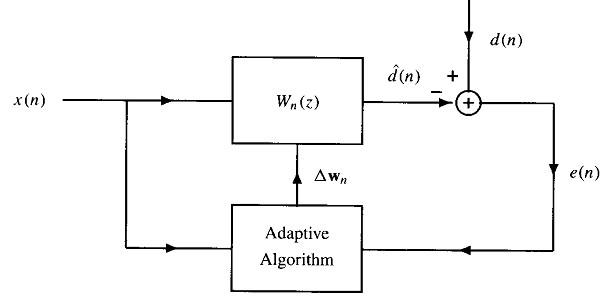
\includegraphics[width=8cm]{./bilder/adaptiveFiltering.jpg}
\end{minipage}
\begin{minipage}{10.5cm}
    \textbf{Goal:} The filter coefficients $w_n$ should be adapted with recursive modification $\Delta w_n$ itself.
    
    \textbf{application area:}
    \begin{liste}
        \item System identification: estimate $H[k], h[n]$ 
        \item Equalize transmission canal  with known sequence: GSM, \ldots
        \item Adaptive noise cancelling (in ear plugs)
        \item Echo cancelling on phone calls
    \end{liste}
\end{minipage}\\
   
The MSE (mean square error) $\xi(w_0, w_1, \ldots, w_n) = E\left(|e(i)|^2\right) = E\left( \left[ d(i) - \sum\limits_{k=0}^{N} w_k x(i-k)\right] ^2 \right)$ should be minimizied. The solution for stationary process is the Wiener-Hopf equations: \\
$$R_x\cdot w = r_{dx}$$
If the process isn't stationary, the filter coefficients have to be updated every step for the optimal result: $w_{n+1}= w_n + \Delta w_n$\\
The adaptive filter should 
\begin{liste}
	\item converge \textbf{to the Wiener-Hopf equations} if the environment is stationary. $\lim\limits_{n\rightarrow\infty} w_n = R_x^{-1}\cdot r_{dx}$
	\item be able to compute the update coefficients $\Delta w_n$, \textbf{without knowledge} of $R_x$ and $r_{dx}$
	\item be able to adapt to the \textbf{changing statistics} and track the solution, if the environment is nonstationary
\end{liste}
\subsubsection{Steepest Descent Adaptive Filter \hayes{499}}
To solve the Wiener-Hopf equations, in every step the autocorrelation matrix has to be inverted and with the crosscorrelation multiplied. 
To reduce this calculations, the coefficient are updated into optimal direction with a small step.
\begin{minipage}{13cm}
$$w_{n+1}=w_n-\mu \cdot  \dfrac{\delta \xi}{\delta w_n} =w_n-\mu \cdot \bigtriangledown\xi(n) \Rightarrow \boxed{ w_{n+1}= w_n+\mu \cdot E\left\lbrace e(n)x^*(n)\right\rbrace}$$ \\
																											$$ \boxed{	w_{n+1}= w_n - \mu \cdot [R_x w_n - r_{dx} ]   }$$ \\
																				%	Stationary solution:	 $ \boxed{	w_{n \to \infty}= w_0 \cdot [R_x w_n - r_{dx} ]^n, n\to \infty   }$
$$ 0<\mu< \frac 2 \lambda_{max}; \lambda_{max} = \text{maximum eigenvalue of autocorrelation matrix } R_x$$
To compute the $E\left\lbrace e(n)x^*(n)\right\rbrace$, a averaging over the last L sample has to be done.  
$$E\left\lbrace e(n)x^*(n)\right\rbrace= \frac{1}{L}\sum\limits_{l=0}^{L-1}e(n-l)x^*(n-l)$$
\end{minipage}
\begin{minipage}{6cm}
        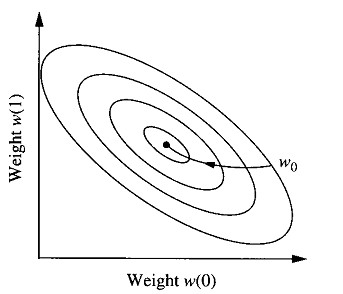
\includegraphics[width=6cm]{../StatDig/bilder/steepestDescent.jpg}
\end{minipage}

 How fast converge the solution/filter: $\displaystyle \tau=\max\{\tau_k\}\approx\frac{1}{\mu \lambda_{min}} $


\clearpage
\subsubsection{LMS Algorithm \hayes{505}}
\begin{minipage}{14cm}

  The LMS algorithm use the same idea as the steepest descent, but just choose the last sample (L=1).\\
  $\boxed{ w_{n+1}=w_n+\mu \cdot e(n) \cdot x^*(n) }$\\
  
  The LMS just converges in the mean, if $\displaystyle 0<\mu< \frac{2}{(p+1)E\left(|x(n)|^2\right)}=\frac{2}{(p+1)r_x(0)}=\frac{2}{(p+1) \cdot \frac{1}{N} \sum\limits_{k=0}^{N-1}|x(n-k)|^2}$.
  The filter coefficients converge to $\hat d(n) = d(n)$ or $e(n) = 0$. 
  That means that filter coefficients always will move, but in the mean they are correct.
\end{minipage}
\begin{minipage}{5cm}
  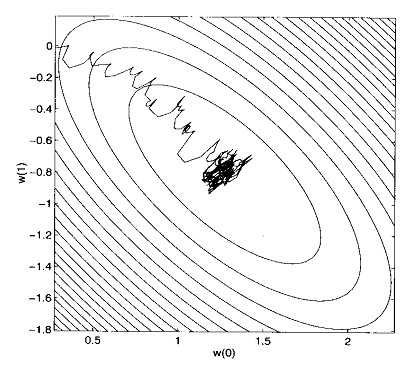
\includegraphics[width=5cm]{../StatDig/bilder/LMS.jpg}
\end{minipage}

\begin{minipage}{9cm}
  \begin{tabbing}
  	Parameters:  \= $p= $ Filter order\\
  	Init:		\> $w_0= 0$\\
  	Computation:
  \end{tabbing}	
      \begin{aufzaehlung}
          \item calculate filter output: $\hat{d}(n) = w_n^T\cdot x(n)$ 
          \item calculate error: $e(n) = d(n) - \hat{d}(n)$
          \item update filter coefficients: $w_{n+1}=w_n+\mu e(n)x^*(n)$  
      \end{aufzaehlung}\vspace{0.05cm}

\end{minipage} 
\begin{minipage}{10cm}
  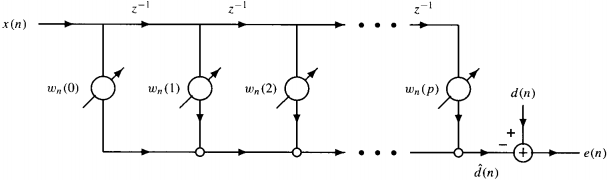
\includegraphics[width=10cm]{../StatDig/bilder/adaptiveFirStructure.png}
\end{minipage}

\subsubsection{Normalized LMS (NLMS) \hayes{514}}
The NLMS is most command used, because it's easy to program, fast to compute and convergence quite fast.\\
The idea is to adapt also the stepsize $\mu(n)=\frac{\beta}{\|x(n)\|^2} \Rightarrow $
$\boxed{w_{n+1}=w_n +\beta \frac{x^*(n)}{\epsilon+\|x(n)\|^2}e(n)}$\\
\begin{liste}
	\item $\|x(n)\|^2$ is the squared sum over $p+1$ samples $\to \sum\limits_{k=0}^{p} | x(n-k) |^2 $, recursively: $\|x(n+1)\|^2 =  \|x(n)\| + |x(n+1)|^2 -|x(n-p)|^2$
 	\item $\epsilon$ is used for small $\|x(n)\|$ (numerical stability)
	\item $\beta$ is a normalized step size with $0 < \beta < 2$
\end{liste}

%Where $\|x(n)\|^2$ is the signal power, $\epsilon$ is used for small $\|x(n)\|$ and is a small positive number and $0<\beta<2$.\\\\
%To reduce the calculation the normalization term $\|x(n)\|$ can also be calculatet recursively:\\ $\|x(n+1)\|^2 =  \|x(n)\| + |x(n+1)|^2 -|x(n-p)|^2$

\subsubsection{Applications - Noise Cancellation \hayes{517}}
\begin{minipage}{9cm}
        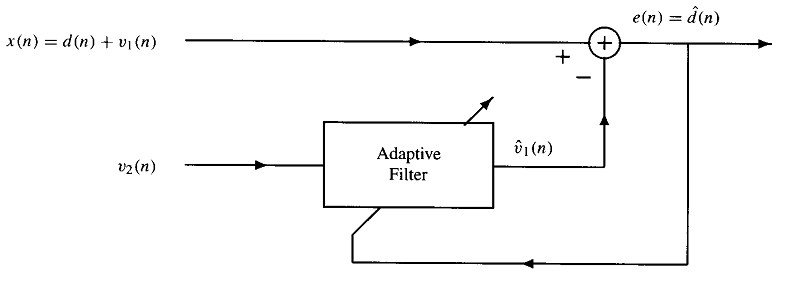
\includegraphics[width=8.5cm]{../StatDig/bilder/adaptiveNoiseCancellation.jpg}\\
        Input signal $x(n)$ with noise (e.g. car noise). 
        The second input measures only the noise (e.g. separate mic). Therefore, $v_1$ and $v_2$ are correlated.
        The filter now guesses the first noise so that the error signal gives the wanted signal $d(n)$.     
\end{minipage}
\hspace{3mm}
\begin{minipage}{9cm}
        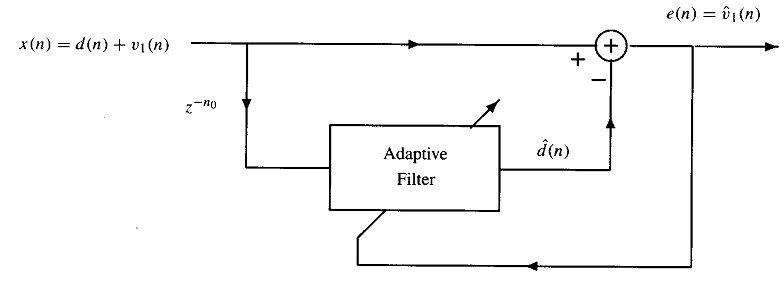
\includegraphics[width=8.5cm]{../StatDig/bilder/NoiseCancellationwithoutRef.jpg}\\
        Input signal $x(n)$ with noise (e.g. car noise). The signal $d(n)$ has to be narrowband and $v_1(n)$ has to be broadband. ($d$ has to be a ``slow''  and $v_1$ has to be a ``fast'' changing signal)
        The filter predicts now $d(n)$ and the error signal is the noise $v_1$.
\end{minipage}

\subsection{Adaptive Recursive Filters (won't be tested) \hayes{534}}
\begin{minipage}{8.4cm}
	Benötigt im Vergleich zum LMS Algorithmus $20M$ nur $2M$ Iterationen bis er konvergiert. RLS nutzt alle vergangene 
	Information zur Berechnung der Korrektur; LMS nutzt nur momentane Information. \\
	$\mathbf{s}(n) = [s(n), s(n-1), \ldots, s(n - N + 1)]^T$ \\
	Forgetting-Faktor ($\mu=1$),
	Initialisierungsfakt. ($\delta = 1)$
\end{minipage}
\begin{minipage}{11cm}
	\begin{aufzaehlung}
	    \item Initialisieren: $n=1; \mathbf{P}(0)=\gamma \cdot \mathbf{I}; \mathbf{\hat{c}}(0)=0$
	    \item Gain Vektor: $ \mathbf{k}(n) = \frac{\mathbf{P}(n-1)\mathbf{s}(n)}{1 + \mathbf{s}^T(n) \mathbf{P}(n-1) \mathbf{s}(n)}$
	    \item Wahrer Schätzfehler: $\eta(n) = r(n) - \mathbf{s}^T(n) \mathbf{\hat{c}}(n-1)$
	    \item Koeffizienten updaten: $\mathbf{\hat{c}}(n) = \mathbf{\hat{c}}(n-1) + \mathbf{k}(n) \eta(n)$
	    \item Fehlerkorrelationsmatrix: \small $\mathbf P(n) = \frac1\mu [ \mathbf P (n-1) - \mathbf k (n) \mathbf u^T (n) \mathbf P(n-1)]$
\normalsize	    \item $n++$ und zurück zu Schritt 2
	\end{aufzaehlung}
\end{minipage}





\end{document}
